\documentclass{article}

\usepackage{arxiv}

\usepackage[utf8]{inputenc}
\usepackage[T1]{fontenc}
\usepackage{hyperref}
\usepackage{url}
\usepackage{booktabs}
\usepackage{amsfonts}
\usepackage{amsmath}
\usepackage{nicefrac}
\usepackage[protrusion=true,expansion=false]{microtype}
\usepackage{graphicx}
\usepackage{natbib}
\usepackage{doi}
\usepackage{array}
\usepackage{tikz}
\usetikzlibrary{shapes.geometric, arrows.meta, positioning, calc}
\usepackage[many]{tcolorbox}
\usepackage{pgfplots}
\pgfplotsset{compat=1.18}
\usepackage{algorithm}
\usepackage{algpseudocode}
\usepackage{enumitem}
\newcommand{\revmark}{\marginpar{\footnotesize\textcolor{blue}{\textbf{Rev.\,2}}}}
\newcommand{\revmarkthree}{\marginpar{\footnotesize\textcolor{red}{\textbf{Rev.\,3}}}}

\title{Semantic Artifact Harness for AI-Native Research\\
{\large Reshaping the Paper Form Through Claims, Algorithms, Code, and Evidence}\\
{\normalsize (Revisiting Loaded Tooth Contact Analysis for Cycloid-Pin-Housing in Robotic Reducers)}}

\author{
OpenCode$^{1}$ \quad Jiacheng Miao$^{2,\ast}$ \\
$^{1}$\texttt{opencode-ai}, \url{https://github.com/opencode-ai/opencode} \\
$^{2}$School of Mechanical Engineering, Dalian Jiaotong University, Dalian 116028, China \\
$^{\ast}$Corresponding author: \texttt{haomjc@163.com}
}

\renewcommand{\shorttitle}{Semantic Artifact Harness}
\renewcommand{\headeright}{\url{https://aixiv.science/abs/aixiv.260429.000001}}

\hypersetup{
pdftitle={Semantic Artifact Harness for AI-Native Research},
pdfsubject={cs.SE, cs.RO},
pdfauthor={Jiacheng Miao},
pdfkeywords={semantic artifact harness, AI-native paper, software engineering for research, algorithm evidence layer, AI-assisted software engineering, reproducible research, robotics, RV reducer, LTCA},
}

\begin{document}
\maketitle

\begin{figure}[t]
\centering
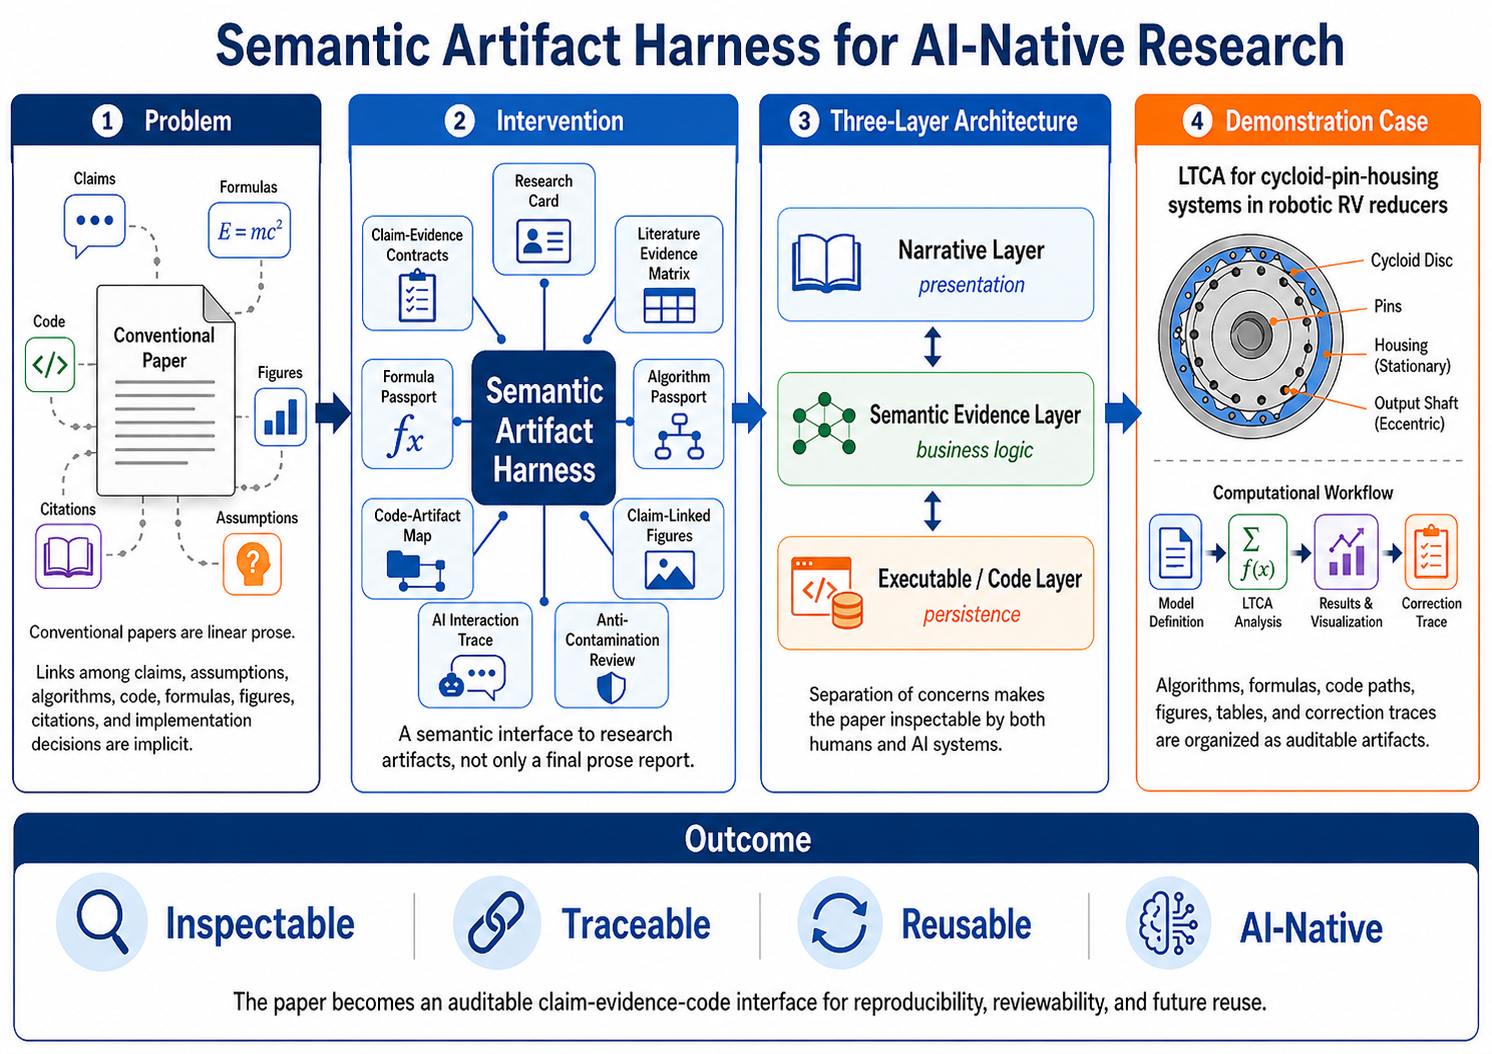
\includegraphics[width=0.95\textwidth]{graphicalAbstract.png}
\caption[Graphical Abstract]{%
\textbf{Graphical Abstract.} An AI-generated overview of the Semantic Artifact Harness architecture: research inputs (data, code, experiments, reasoning) flow through the three-layer harness (narrative, semantic evidence, executable), producing an inspectable research artifact with typed interfaces. This figure was generated by GPT Image 2 based on a natural-language prompt describing the paper's core argument and structure. The prompt specified the layout, color scheme, and labeled components; the researcher reviewed and approved the output.}
\label{fig:graphical_abstract}
\end{figure}

\begin{abstract}
\textbf{Problem.}
Most research papers still follow a linear narrative format designed for human reading. This format is increasingly mismatched with how papers are now consumed: AI systems search, summarize, compare, verify, review, and reuse scientific claims before any human reads them. Conventional prose hides the links among claims, assumptions, algorithms, code, formulas, figures, citations, and implementation decisions. The resulting risk is an AI-to-AI contamination loop: AI writes papers, AI reads them, AI reviews them, databases index them, and later AI systems retrieve or train on the accumulated output. In that loop, errors do not disappear---they become more stable because they are repeated in a scholarly style. Without explicit norms and constraints for AI-native research artifacts, fluent but wrong contributions become harder to detect as they propagate through the literature.

\textbf{Intervention.}
This paper proposes the \emph{Semantic Artifact Harness}: a paper form that treats the manuscript as a typed program with explicit interfaces rather than as a final prose report. The design applies software engineering norms---contracts, test harnesses, API specifications, separation of concerns, supply-chain integrity, and CI/CD-style verification---as explicit constraints for AI-native research artifacts. The goal is to make every claim auditable, every evidence link traceable, every algorithm inspectable, and every limitation machine-readable, so that the AI-to-AI contamination loop can be broken.

\textbf{Framework.}
The harness is organized into three layers---narrative (presentation), semantic evidence (business logic), and executable/code (persistence)---following the separation-of-concerns principle. Its central components are research cards, claim-evidence contracts, dense literature evidence matrices, formula passports, algorithm passports, code-artifact maps, claim-linked figures, compressed AI-interaction traces, and an anti-contamination review protocol. A verification ladder establishes explicit norms: each research claim must pass through layers of verification (formal proof, code execution, numerical simulation, experiment, embodied interaction, literature feedback) before being promoted. In this structure, algorithms, literature context, implementation paths, failure checks, and verification stage all become first-class evidence objects, not supplementary descriptions.

\textbf{Demonstration.}
The format is demonstrated through a loaded tooth contact analysis (LTCA) program for cycloid-pin-housing systems in robotic RV reducers. The manuscript itself is used as a self-bootstrapping AI-assisted artifact: its code inspection, manuscript structure, tables, figures, literature matrices, BibTeX records, and correction traces were iteratively generated, reorganized, and audited through human--AI interaction. The case demonstrates that SE practices---contract-driven design, interface specification, regression testing, and supply-chain integrity---transfer naturally to computational research artifacts, even though the primary output remains a reshaped research paper.
\end{abstract}

\keywords{semantic artifact harness; AI-native paper; software engineering for research; algorithm evidence layer; claim graph; reproducible research; AI-assisted software engineering; RV reducer; loaded tooth contact analysis}

\section*{Research Card}

\begin{center}
\begin{tabular}{p{3.0cm}p{10.5cm}}
\toprule
\textbf{Object} & A semantic artifact harness for AI-native computational engineering papers. \\
\textbf{Case substrate} & Loaded tooth contact analysis for cycloid-pin-housing systems in robotic RV reducers. \\
\textbf{Core claim} & A research paper should not only report a final model; it should expose a structured engineering interface that connects claims, assumptions, algorithms, code, formulas, figures, evidence, limitations, corrections, and anti-contamination checks---analogous to how software engineering makes complex systems inspectable through contracts, tests, and audit trails. \\
\textbf{Primary audience} & Human researchers, AI readers, reviewers, and future reuse agents. \\
\textbf{Evidence types} & Claim maps, dense literature matrices, algorithm passports, pseudocode, flowcharts, Git commits, MATLAB source files, formula audits, LaTeX source, BibTeX records, and generated figures. \\
\textbf{Known limits} & The case model is quasi-static LTCA. It does not replace full transient tribo-dynamics, elastohydrodynamic lubrication, asperity-contact wear evolution, thermal modeling, or physical experiment. The harness improves auditability; it does not prove correctness by appearance. \\
\bottomrule
\end{tabular}
\end{center}

\section{Why the Paper Form Must Change}

The conventional research paper is optimized for a human reader moving from title to abstract, introduction, methods, results, and conclusion. This form is useful, but it is no longer sufficient. In current research practice, a paper is frequently read by AI systems before, during, and after human reading. AI systems extract claims, map citations, compare methods, locate formulas, inspect code, and generate summaries. The traditional manuscript gives these systems long prose but weak structure.

This is, at its core, a software engineering problem. The research paper is a system---no different from a program or a function---with multiple stakeholders (authors, reviewers, AI agents, future reusers), multiple interfaces (prose, code, data, figures, citations), and no specification language that makes the system testable. Just as a function without a signature, return type, and error contract is hard to reuse, a paper without explicit claims, evidence links, and boundary conditions is hard to audit. Software engineering has already developed discipline for making complex systems inspectable: contracts, test harnesses, type systems, API documentation, version control, code review, supply-chain security, and CI/CD pipelines. The question this paper asks is: what happens when these practices are transferred to the research paper itself? The answer is that the paper should be treated not as a final prose report, but as an inspectable artifact with typed interfaces---a program that exposes its claims, assumptions, algorithms, and evidence through structured, machine-readable contracts.

The problem is not that prose is useless. Prose remains necessary for argument, context, and judgment. The problem is that prose is often the only carrier of information. A claim may be stated in the abstract, supported by a figure, implemented in a source file, derived from a formula, and constrained by assumptions hidden in code. In a conventional paper, these links are implicit. In an AI-native paper, they should be explicit.

This paper therefore treats the manuscript as a research interface rather than a static report. The interface should allow a human or AI reader to answer several questions quickly:

\begin{itemize}
    \item What exactly is claimed?
    \item Which code or calculation supports the claim?
    \item Which formula implements the physical assumption?
    \item Which AI-suggested changes were accepted, rejected, or corrected by the researcher?
    \item Which parts are validated, and which are outside the scope?
\end{itemize}

We call this design practice the \emph{Semantic Artifact Harness}. The term is borrowed from software engineering: a test harness surrounds a program with the scaffolding needed to run, observe, and verify it. Analogously, an artifact harness surrounds a research model with the scaffolding needed to inspect, reproduce, challenge, and reuse it. The harness is not the scientific contribution alone; it is the engineered structure that makes the contribution reviewable. Like a test harness, it separates the system under test (the scientific model) from the scaffolding (claims, contracts, verification stages, failure checks) that makes it inspectable.

Furthermore, AI assistants can significantly elevate the typographic presentation of the manuscript. A raw dump of text is hard for human readers to parse. By leveraging AI to automatically structure content into rich LaTeX elements---such as styled summary cards using \texttt{tcolorbox}, logical workflow flowcharts using \texttt{TikZ}, and meticulously formatted tables---the manuscript achieves a level of visual clarity that greatly enhances human readability. The paper is no longer just a wall of text, but a visually structured communication tool that guides the reader's attention to critical claims, formulas, and artifacts.

This also changes the meaning of figures, tables, and data display. Many current journal papers use polished multi-panel figures, dense plots, and elaborate tables as signals of completeness. In an AI-mediated reading environment, however, a beautiful figure that is not linked to data, code, parameters, and claims becomes a decorative endpoint: it attracts attention while hiding provenance. The solution is not to replace the paper with a raw open data package. Data packages are necessary, but by themselves they often lack interpretation, model boundaries, failure cases, and the author's reason for trusting one view over another.

The better target is a role shift: figures and tables should become \emph{evidence interfaces}. They should remain readable to humans, but each visual object should also point to the data subset, generation script, parameter range, validation check, and claim ID that make it auditable by AI.

\begin{tcolorbox}[title=Role Shift of Visual Evidence in an AI-Native Paper, colback=white, colframe=gray!60!black]
\small
\setlength{\tabcolsep}{3pt}
\begin{tabular}{p{3.0cm}p{4.2cm}p{5.8cm}}
\toprule
\textbf{Conventional object} & \textbf{AI-era risk} & \textbf{Harness role} \\
\midrule
Polished schematic & Persuasive decoration without provenance & Link geometry, assumptions, claim IDs, and regeneration path. \\
Dense plot & High visual load with unclear source data & Expose plotted data, script, parameter sweep, and selection rule. \\
Large table & Human-readable but hard to query or reuse & Convert to a compact view of a machine-readable evidence matrix. \\
Open data package & Transparent but under-interpreted & Bind files to research cards, model boundaries, and validation questions. \\
Narrative prose & Easy to read but weak for verification & Preserve as the judgment layer that explains why evidence was selected. \\
\bottomrule
\end{tabular}
\end{tcolorbox}

Human reading therefore remains important, but its purpose changes. The human reader should not be forced to absorb every plotted curve, table entry, or supplementary file. Human reading should focus on judgment: whether the research question is meaningful, whether the model boundary is defensible, whether the displayed evidence is representative, and whether AI-generated structure has been corrected by domain expertise.

\section{From IMRaD Writing to AI-Native Research Workflow}

The conventional IMRaD pattern is useful for final narration, but inefficient as a working process. Authors often write introduction, method, result, and discussion sections before the research artifacts are fully aligned. This creates repeated rewriting: references are rearranged, claims are softened, figures are redrawn, and formulas are explained in prose because the paper has no explicit artifact structure.

The harness changes the order of work. Instead of starting from section prose, the author first builds a standardized research workflow:

\begin{enumerate}
    \item Define the research object, scope, excluded physics, and expected outputs.
    \item Ask AI to inspect the repository, identify executable entry points, and map code artifacts.
    \item Build a claim-evidence map before writing long prose.
    \item Convert key algorithms into passports, pseudocode, flowcharts, and code-path maps.
    \item Convert literature into a dense evidence matrix rather than a long chronological review.
    \item Generate figures and tables from scripts whenever possible.
    \item Record the optimization trace: human question, AI analysis, author judgment, artifact changed, and rebuild result.
    \item Write the narrative layer after the semantic and executable layers are stable.
\end{enumerate}

This workflow treats AI as a builder and auditor of the artifact harness, not merely as a prose generator. The author still makes the scientific judgment, but the repetitive work of extracting structure, checking consistency, formatting evidence, and rebuilding the manuscript can be delegated to AI-assisted tools.

The pattern is not limited to MATLAB-based analysis. The same natural-language-driven workflow now extends across computational engineering domains. For example, fluid--structure interaction problems that once required manual mesh generation, solver configuration, and coupling setup can be addressed by instructing an AI agent to install and configure preCICE \citep{chourdakis2022preCICE} as a coupling library between OpenFOAM (CFD) \citep{openfoam} and CalculiX (FEM) \citep{dhondt2024calculix} within a Linux subsystem, define boundary conditions, run the partitioned simulation, and extract results---all through natural language without writing a single solver configuration file manually. Similarly, multibody dynamics frameworks such as Exudyn \citep{holzinger2024exudyn} allow AI agents to construct theoretical extensions, script automated models, and partially validate analytical predictions against numerical simulations. These examples suggest that the Semantic Artifact Harness is not tied to a single tool or discipline: any computational workflow in which AI mediates between researcher intent and solver execution can benefit from the same claim--evidence--code structure.

\section{Semantic Artifact Harness Architecture}

Semantic Artifact Harness engineering keeps ordinary LaTeX and PDF compatibility, but adds structural layers that make the paper easier to inspect, query, and reuse. The paper becomes a harness around the research object: it connects otherwise scattered artifacts and exposes their relationships.

\subsection{Harness Architecture: Three Layers}

The harness is organized as three mutually linked layers. The human narrative layer preserves explanation and scientific judgment. The semantic evidence layer turns claims, algorithms, formulas, figures, assumptions, and limitations into identifiable objects. The executable/code layer keeps the computational substrate available for inspection and regeneration.

\begin{table}[t]
\caption{Three-layer architecture of the Semantic Artifact Harness.}
\centering
\small
\begin{tabular}{p{3.2cm}p{4.8cm}p{5.1cm}}
\toprule
\textbf{Layer} & \textbf{Human role} & \textbf{AI-readable role} \\
\midrule
Narrative layer & Explains motivation, domain judgment, and interpretation. & Provides prose context for claim extraction and summarization. \\
Semantic evidence layer & Organizes claims, assumptions, formulas, algorithms, figures, risks, and limits. & Provides stable objects that can be queried, compared, and audited. \\
Executable/code layer & Holds scripts, data, source files, parameters, and rebuild commands. & Allows code-path inspection, figure regeneration, and consistency checks. \\
\bottomrule
\end{tabular}
\label{tab:layers}
\end{table}

The key design choice is that the PDF is only one view of the paper. The LaTeX source, tables, code references, generated data, and figure scripts together form the research interface. A future implementation could also emit a machine-readable manifest, but the present paper keeps the idea deployable using standard LaTeX, BibTeX, Git, and source files.

The three-layer architecture follows the separation-of-concerns principle familiar from software architecture: the narrative layer is the presentation (view), the evidence layer is the business logic (model), and the executable layer is the persistence (data). The paper itself is a program: it takes raw research (data, code, experiments, reasoning) as input and produces a claim--evidence structure as output. In the AI era, this program is no longer consumed only by human readers. AI agents need to call its interfaces---extract claims, trace citations, verify formulas, reproduce results---without reading the entire source. Standardizing these interfaces is therefore not an aesthetic improvement; it is an interoperability requirement.

\subsection{Software Engineering Foundations}

The artifact harness can be understood as a transfer of established software engineering patterns to research paper construction. Table~\ref{tab:se_mapping} makes this mapping explicit.

\begin{table}[t]
\caption{Mapping between artifact harness concepts and software engineering patterns.}
\centering
\small
\begin{tabular}{p{3.6cm}p{3.6cm}p{5.5cm}}
\toprule
\textbf{Harness concept} & \textbf{SE equivalent} & \textbf{Shared purpose} \\
\midrule
Claim-evidence map & Design by Contract & Pre/post-conditions per unit of contribution. \\
Algorithm passport & API documentation (OpenAPI) & Interface signature, inputs, outputs, and error modes. \\
Formula passport & Type signature & Units as types; dimensions as invariants. \\
Three-layer architecture & Separation of concerns (MVC) & View / business logic / persistence. \\
Model-evolution log & Version control (Git) & Commit history as audit trail. \\
AI-interaction trace & Code review record & Reviewer, decision, and changed files are preserved. \\
Anti-contamination protocol & Supply-chain security & Dependency poisoning prevention. \\
Verification ladder & CI/CD pipeline & Each rung is a gate that must pass before promotion. \\
Evidence-weighted database & Package registry with trust scores & npm advisory / Sigstore provenance. \\
\bottomrule
\end{tabular}
\label{tab:se_mapping}
\end{table}

This mapping is not decorative. Software engineering has spent decades solving the problem of how to make complex systems auditable by people who did not write them. Research papers face the same problem: a reviewer, an AI reader, or a future reuser must assess claims without having watched the research process. The harness borrows the solution strategy---structured interfaces, typed contracts, automated checks, and recorded provenance---and applies it to the paper itself.

More concretely, a paper can be viewed as a function with a typed interface. Its inputs are assumptions, prior knowledge, datasets, and code; its outputs are claims, evidence, and boundary conditions. The harness adds the function signature: for each claim, what are the preconditions (assumptions, valid parameter ranges), the postconditions (verified predictions, confirmed measurements), and the failure modes (cases where the claim does not hold)? Without this signature, an AI system that reads the paper cannot safely call its claims as building blocks for new work. It must first reverse-engineer the contract---an expensive and error-prone process. Standardizing the paper as a typed artifact therefore serves the same purpose as standardizing an API: it makes downstream composition safe, efficient, and auditable.

\subsection{Harness Interface: Research Card}

The research card is a front-page index. It is not a replacement for the abstract. It is a compact map of the research object. A reviewer or AI system can use it to identify the main claim, artifact types, scope, and limitations before reading any long section.

\subsection{Harness Interface: Structured Abstract}

The abstract is split into \texttt{Problem}, \texttt{Intervention}, \texttt{Case Study}, and \texttt{Claim}. This removes ambiguity about whether the paper's contribution is a physical model, a software workflow, or a writing method. For this paper, the case study concerns RV reducer LTCA, but the methodological claim concerns AI-assisted computational research.

\subsection{Harness Connectors: Claim-Evidence Map}

Each major claim is paired with its evidence artifact. Table~\ref{tab:claim_map} shows the claim-evidence structure used in this manuscript.

\begin{table}[t]
\caption{Claim-evidence map for the artifact harness.}
\centering
\small
\begin{tabular}{p{3.3cm}p{5.0cm}p{5.0cm}}
\toprule
\textbf{Claim} & \textbf{Evidence artifact} & \textbf{Inspection path} \\
\midrule
The paper should operate as a semantic interface, not only as prose. & Three-layer harness architecture in Table~\ref{tab:layers}. & Check whether narrative, evidence, and code layers are explicitly connected. \\
Algorithms should be first-class evidence objects. & Algorithm passport, pseudocode, and flowchart in Section~\ref{sec:algorithm_layer}. & Trace each algorithm step to assumptions, outputs, code paths, and claims. \\
Literature should be compressed into reusable evidence. & Dense literature evidence matrix in Table~\ref{tab:literature_matrix}. & Check which source supports which modeling role, boundary, or comparison target. \\
AI assistance requires human physical judgment. & Curvature correction and floating-pin reinterpretation in Table~\ref{tab:evolution}. & Compare AI-proposed changes against researcher corrections. \\
The case is a substrate for harness construction, not the only contribution. & LTCA model-evolution log and artifact map. & Inspect how the same harness pattern could be reused outside this mechanism case. \\
\bottomrule
\end{tabular}
\label{tab:claim_map}
\end{table}

\subsection{Harness Connectors: Algorithm Evidence Layer}
\label{sec:algorithm_layer}

In a Semantic Artifact Harness, algorithms are not supplementary explanations. They are first-class evidence objects that bind claims, assumptions, equations, code, figures, and failure modes. A conventional paper may provide pseudocode as a compact description. A harnessed paper should additionally explain why the algorithm exists, which claim it supports, where it is implemented, what it consumes, what it produces, and how it can fail.

\begin{tcolorbox}[colback=orange!4!white,colframe=orange!70!black,title=Algorithm Passport: Loaded Contact Solver,arc=4mm,boxrule=1pt]
\small
\begin{tabular}{>{\bfseries}p{3.0cm}p{10.5cm}}
\toprule
ID & ALG-LTCA-Force-Balance. \\
Purpose & Solve loaded contact force distribution under clearance, compliance, tooth-body stiffness, and static friction. \\
Supports claims & Floating-pin clearance must be consumed before elastic pin-housing compression; algorithmic claims must be linked to code paths and visual evidence. \\
Inputs & Geometry, profile data, pin radius, housing-hole radius, clearance, stiffness parameters, friction coefficient, and external torque. \\
Outputs & Contact forces, contact count, transmission error, torque residual, and geometry points for figure generation. \\
Implemented in & \texttt{fun\_force.m}, with stiffness support from \texttt{fun\_tooth\_stiffness.m} and data export through \texttt{export\_tikz\_data.m}. \\
Iterative core & Output displacement, pin-hole relative motion, clearance consumption, pin-housing contact deformation, tooth compliance, and force balance are updated together until the torque residual and contact state stabilize. \\
Assumptions & Quasi-static equilibrium, small deformation, dominant normal contact, and static friction represented through equivalent torque projection. \\
Failure modes & Narrow torque-balance root window, confused radius definitions, treating clearance as elastic compression too early, fixed-pin assumptions hiding pin motion, and non-contact placeholders entering numerical aggregation. \\
\bottomrule
\end{tabular}
\end{tcolorbox}

\begin{tcolorbox}[colback=gray!3!white,colframe=gray!65!black,title=Pseudocode Evidence: Harnessed LTCA Solver,arc=4mm,boxrule=1pt]
\small
\begin{enumerate}
    \item Read geometry parameters and separate profile-generation radius, actual pin radius, and housing-hole radius.
    \item Compute unloaded contact candidates and their local geometric approach.
    \item For each candidate, compute relative motion between actual pin center and housing-hole center.
    \item Consume rigid pin-housing clearance before assigning elastic pin-housing compression.
    \item Assemble Hertz contact stiffness, tooth-body stiffness, optional pin stiffness, and pin-housing compliance in series.
    \item Iteratively solve output displacement, pin-hole contact deformation, and global torque equilibrium using bracketed root search when necessary.
    \item Update normal force, friction contribution, contact count, transmission error, and pin-hole contact state.
    \item Export contact point, pin center, housing-hole center, and plotted boundaries for claim-linked figures.
    \item Record failure modes and accepted corrections in the model-evolution log.
\end{enumerate}
\end{tcolorbox}

The algorithm passport above describes the logic. A stronger form---required by the SE mapping in Table~\ref{tab:se_mapping}---adds formal pre/post-conditions and convergence analysis. Crucially, every claim below was verified against the actual source code (\texttt{runTCA\_analysis.m} and \texttt{fun\_force\_analysis.m}); nothing was inferred from the algorithm description alone.

\revmark % Rev.2: Formal specification expanded with code-verified pre/post-conditions
\revmarkthree % Rev.3: Runtime assertions, JSON Schema, and Dafny contracts published to GitHub
The algorithm passport above describes the logic. A stronger form adds formal pre/post-conditions and convergence analysis. In version~3.0, these were further extended into machine-verifiable contracts: MATLAB runtime assertions (\texttt{SAH\_PRE}/\texttt{SAH\_POST}/\texttt{SAH\_CONV} in \texttt{fun\_force\_analysis.m}), a JSON Schema for the harness structure, and a Dafny contract sketch with loop invariants. The full formal specification, including code-verified preconditions, postconditions, root-finding strategy, pin-hole iteration convergence, and numerical stability analysis, is provided in Appendix~\ref{sec:app_formal}.

\begin{figure}[t]
\centering
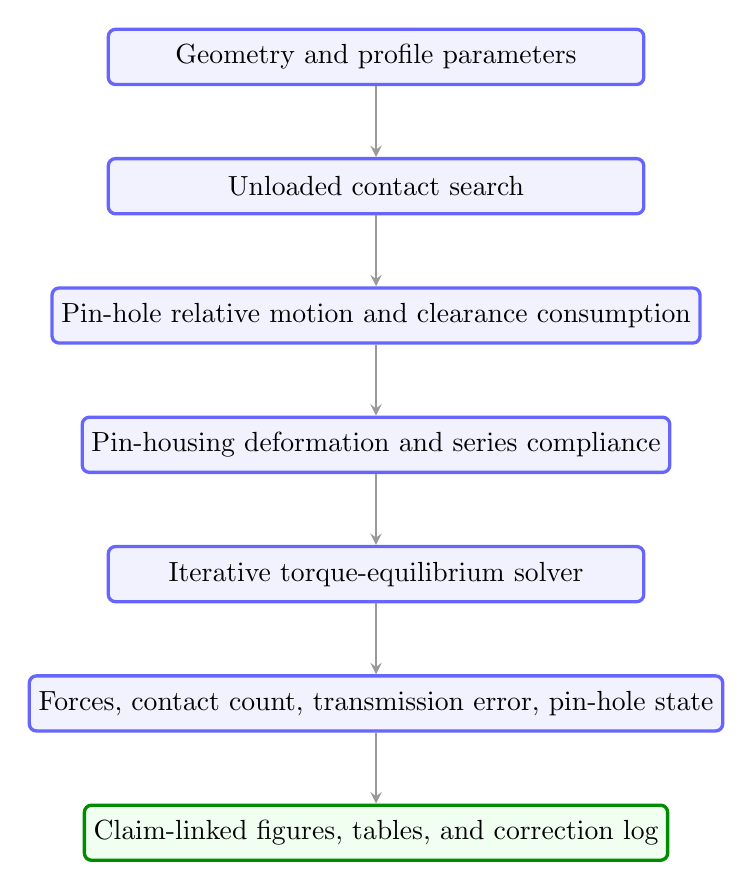
\begin{tikzpicture}[
    node distance=0.9cm,
    flowstep/.style={rectangle, draw=blue!60, fill=blue!5, very thick, minimum width=6.8cm, minimum height=0.7cm, align=center, rounded corners=0.6ex},
    evidence/.style={rectangle, draw=green!55!black, fill=green!6, very thick, minimum width=6.8cm, minimum height=0.7cm, align=center, rounded corners=0.6ex},
    arrow/.style={->, >=stealth, thick, draw=gray!80}
]
\node (geom) [flowstep] {Geometry and profile parameters};
\node (contact) [flowstep, below=of geom] {Unloaded contact search};
\node (clearance) [flowstep, below=of contact] {Pin-hole relative motion and clearance consumption};
\node (stiffness) [flowstep, below=of clearance] {Pin-housing deformation and series compliance};
\node (solver) [flowstep, below=of stiffness] {Iterative torque-equilibrium solver};
\node (outputs) [flowstep, below=of solver] {Forces, contact count, transmission error, pin-hole state};
\node (evidence) [evidence, below=of outputs] {Claim-linked figures, tables, and correction log};
\draw [arrow] (geom) -- (contact);
\draw [arrow] (contact) -- (clearance);
\draw [arrow] (clearance) -- (stiffness);
\draw [arrow] (stiffness) -- (solver);
\draw [arrow] (solver) -- (outputs);
\draw [arrow] (outputs) -- (evidence);
\end{tikzpicture}
\caption{\textbf{Algorithm flowchart as evidence.} Claim: the algorithm is a semantic bridge between theory, code, and manuscript evidence. Inspect: whether each stage has corresponding variables, assumptions, failure modes, and generated artifacts.}
\label{fig:algorithm_flow}
\end{figure}

\subsection{Harness Connectors: Formula Passport}

Formulas should not appear as isolated mathematical objects, but the harness also should not over-explain every equation. Only decision-critical formulas need passports: formulas that control a claim, define an algorithmic branch, map directly to source code, or are likely to be physically misinterpreted. The following stiffness combination is used as an example:

\begin{tcolorbox}[colback=blue!5!white,colframe=blue!75!black,title=Formula Passport: Effective Normal Stiffness,arc=4mm,boxrule=1pt]
\begin{equation}
    K_{\mathrm{total}} =
    \frac{1}{1/K_h + 1/K_g + 1/K_r + 1/K_{ph}},
    \label{eq:series_stiffness}
\end{equation}
where $K_h$ is cycloid-pin Hertz stiffness, $K_g$ is cycloid tooth-body stiffness, $K_r$ is pin structural stiffness if included, and $K_{ph}$ is pin-housing elastic stiffness after clearance is consumed.

\vspace{2mm}
\small
\begin{tabular}{>{\bfseries}p{3.0cm}p{10.5cm}}
\toprule
Role & Converts multiple local deformation mechanisms into one effective normal stiffness. \\
Inputs & Hertz contact, tooth-body bending/shear/compression, optional pin stiffness, and pin-housing compliance. \\
Units & N/mm when all component stiffnesses are in N/mm. \\
Code path & \texttt{fun\_force.m} for LTCA force balance; \texttt{fun\_tooth\_stiffness.m} for $K_g$. \\
Failure mode & Invalid if clearance is treated as elastic compression before rigid gap consumption. \\
Human correction & Researcher clarified that a smaller pin moves inside a larger housing hole before elastic compression develops. \\
\bottomrule
\end{tabular}
\end{tcolorbox}

\subsection{Harness Connectors: Dense Literature Evidence Matrix}

Traditional literature reviews are costly to write and costly to parse. They often spend many paragraphs rephrasing source papers while hiding the key information needed by a reader or AI system: what role the source plays, which claim it supports, what it contributes, and where its boundary lies. A Semantic Artifact Harness therefore treats literature as a structured evidence layer. Full citation metadata remains in BibTeX, but the manuscript presents a dense literature matrix that maximizes information per line.

\begin{tcolorbox}[colback=yellow!4!white,colframe=yellow!55!black,title=AI-Assisted Literature Collection Protocol,arc=4mm,boxrule=1pt]
\small
The literature layer was built as a traceable AI-assisted search rather than a conventional paragraph-by-paragraph review. The seed queries combined \emph{cycloid-pin}, \emph{cycloid pinwheel}, \emph{cycloidal reducer}, \emph{RV reducer}, \emph{TCA}, \emph{LTCA}, \emph{loaded tooth contact}, \emph{assembling clearance}, \emph{pin load sharing}, \emph{profile modification}, \emph{lost motion}, \emph{tooth wear}, and \emph{isogeometric contact}. Search results and citation chains were grouped by modeling role rather than by chronology: geometry/profile design, clearance and multi-pin contact, loaded contact analysis, stiffness and compliance, wear/tribology, lost-motion validation, and high-fidelity dynamic or finite-element boundary models. The author then inspected this grouping to decide which papers support the harness demonstration, which papers define its boundary, and where this work differs from fixed-pin TCA assumptions.
\end{tcolorbox}

\begin{table}[t]
\caption{Dense literature evidence matrix for geometry, clearance, and LTCA/contact calculation.}
\centering
\small
\begin{tabular}{p{2.7cm}p{3.0cm}p{3.7cm}p{3.8cm}}
\toprule
\textbf{Source} & \textbf{Modeling role} & \textbf{Reusable information} & \textbf{Harness use} \\
\midrule
\citet{sensinger2010optimization} & Profile, stress, and efficiency optimization. & Unified view of cycloid profile, stress, and efficiency tradeoffs. & Supports treating geometry as a decision-critical artifact. \\
\citet{ivanovic2012clearances} & Trochoidal meshing with clearances. & Clearance changes meshing state and should not be hidden in prose. & Motivates explicit clearance objects in the harness. \\
\citet{lin2014twostage} & Tooth modification for cycloidal reducers. & Profile modification affects transmission behavior and geometry. & Supports profile data as an artifact, not only a formula. \\
\citet{xu2016dynamic} & Dynamic contact analysis of cycloid-pin mechanism. & Multi-pin contact and bearing coupling under dynamic formulation. & Provides contrast to the lower-cost quasi-static LTCA harness. \\
\citet{yang2018stiffness} & Cycloid-pin meshing stiffness. & Energy-method basis for tooth-body compliance. & Supports the need for a stiffness passport and code mapping for $K_g$. \\
\citet{tsai2017ltca} & LTCA with friction and bearing roller stiffness. & Loaded contact requires coupling friction, bearing stiffness, and contact state. & Supports algorithm passport for coupled force-balance logic. \\
\citet{li2017clearancefit} & Profile modification and clearance-fit output mechanism. & Clearance-fit output behavior is a design variable, not a nuisance term. & Supports modeling clearance and output motion explicitly. \\
\citet{xu2019assembling} & Pin load sharing with assembling clearance. & Number of load-transmitting pins changes under clearance. & Directly supports the need to audit contact-count collapse. \\
\citet{wang2019transmission} & RV reducer transmission performance. & Load and profile modification affect transmission error and meshing force. & Positions the case within RV reducer performance analysis. \\
\citet{sun2019cbr} & Loaded tooth contact analysis of China Bearing Reducer. & Modification and LTCA can be organized as a design workflow. & Supports reuse of the harness beyond the present RV case. \\
\citet{sun2024cbrtca} & CBR TCA with modification and manufacturing error. & TCA can be combined with B-spline reconstructed profile errors and optimization. & Shows how TCA evidence can be extended to error-aware profile design. \\
\bottomrule
\end{tabular}
\label{tab:literature_matrix}
\end{table}

\begin{table}[t]
\caption{Dense boundary and validation matrix for dynamic, wear, lost-motion, and high-fidelity contact studies.}
\centering
\small
\begin{tabular}{p{2.7cm}p{3.0cm}p{3.7cm}p{3.8cm}}
\toprule
\textbf{Source} & \textbf{Modeling role} & \textbf{Reusable information} & \textbf{Harness use} \\
\midrule
\citet{sun2018lostmotion} & Lost-motion analysis of a cycloid-pin reducer. & Initial gap, modification, machining error, and hysteresis testing are connected. & Links clearance modeling to measurable precision-reducer behavior. \\
\citet{xu2019lostmotion} & Dynamic lost-motion measurement. & Measurement speed, friction, and geometric lost motion should be separated. & Provides a validation-oriented metric for future harness extension. \\
\citet{xu2019bcptm} & Dynamic contact of bearing-cycloid-pinwheel mechanisms. & Cycloid-pin backlash and bearing clearance affect dynamic load transmission. & Defines a higher-fidelity dynamic boundary beyond the quasi-static harness. \\
\citet{li2023dynamicrv} & RV reducer dynamics using LTCA-derived mesh quantities. & Equivalent mesh stiffness and pressure angle can be built from loaded contact analysis. & Connects LTCA evidence to whole-reducer dynamic modeling. \\
\citet{li2023wearprofile} & Wear with profile modification. & LTCA provides contact stress and sliding inputs for Archard wear prediction. & Shows how the harness can extend from contact load to wear. \\
\citet{wang2023ltca} & Loaded contact and wear analysis. & Elimination-clearance LTCA, quasi-Hertz contact, contact count, and wear calculation. & Supports design-stage LTCA while highlighting that pin-hole motion must be exposed separately. \\
\citet{zhang2023iga} & Isogeometric finite-element contact analysis. & High-continuity NURBS geometry can improve contact-stress calculation efficiency. & Provides a high-fidelity benchmark path for future validation of contact pressure. \\
\citet{li2025tribodynamics} & Transient tribo-dynamics. & Higher-fidelity scope including transient effects beyond quasi-static LTCA. & Defines the boundary of the present harness demonstration. \\
\bottomrule
\end{tabular}
\label{tab:boundary_matrix}
\end{table}

This matrix does not replace scholarship. It replaces low-density citation prose with an inspectable citation object. AI can compare sources by role, authors can check whether each citation has a reason to exist, and reviewers can see whether the paper is using a source as model basis, contrast case, validation target, or boundary condition.

\subsection{Harness Precedents: Paper Form and Research Objects}
\label{sec:app_precedents}

The Semantic Artifact Harness is not proposed in isolation. It extends several earlier attempts to improve scientific communication. IMRaD standardized the narrative order of biomedical articles \citep{sollaci2004imrad}, while genre-analysis work such as the CARS model explains how research articles create rhetorical space for a contribution \citep{swales1990genre}. Literate programming argued that code should be written for human explanation as well as machine execution \citep{knuth1984literate}. Executable-paper systems and virtual research environments moved papers closer to runnable artifacts \citep{vanGorp2011share,leBorgne2011openreview}. Research Objects and FAIR principles further shifted attention from a paper as text to a shareable, reusable, and machine-actionable bundle of knowledge resources \citep{bechhofer2010researchobjects,wilkinson2016fair}.

\begin{table}[t]
\caption{Paper-form and research-object precedents for the artifact harness.}
\centering
\small
\begin{tabular}{p{2.7cm}p{3.4cm}p{3.7cm}p{3.6cm}}
\toprule
\textbf{Precedent} & \textbf{Primary contribution} & \textbf{Limitation for AI-native research} & \textbf{Harness extension} \\
\midrule
\citet{sollaci2004imrad} & Historical survey of IMRaD standardization. & Organizes narrative but not code, claims, or AI traces. & Keeps readable prose but adds evidence objects. \\
\citet{swales1990genre} & Rhetorical move structure for research articles. & Explains persuasion, not executable verification. & Converts contribution moves into claim-evidence maps. \\
\citet{knuth1984literate} & Integrates program and explanation. & Focuses on code comprehension more than literature, review, or experimental evidence. & Treats algorithms and code paths as manuscript evidence. \\
\citet{vanGorp2011share} & Virtual machines for executable papers. & Helps reproduce computations but not claim-level audit. & Adds semantic links among claims, code, formulas, and limits. \\
\citet{leBorgne2011openreview} & Post-publication executable-paper review. & Centers on reproducibility incentives and executable annotations. & Adds AI-readable anti-contamination checks. \\
\citet{bechhofer2010researchobjects} & Research Objects as reusable knowledge bundles. & Resource aggregation may still lack domain-specific claim audits. & Defines claim, formula, algorithm, figure, and correction passports. \\
\citet{wilkinson2016fair} & FAIR principles for data stewardship. & Data can be FAIR without proving the paper's argument. & Applies machine-actionability to claims and validation state. \\
\bottomrule
\end{tabular}
\label{tab:paper_form_precedents}
\end{table}

The harness therefore differs from a conventional template. It is closer to an engineered interface for research evidence. Its central question is not only ``How should the paper be written?'' but ``What must be exposed so that a human, AI reader, AI reviewer, or future autonomous research system can detect unsupported claims before they enter the literature?''

\subsection{Harness Trace: AI-Interaction Record}

An artifact harness should not hide AI involvement, but it also should not dump raw chat logs. The useful unit is a compressed interaction trace: human challenge, AI action, accepted correction, and artifact changed. This preserves accountability and exposes where domain expertise entered the loop. In software engineering terms, this is analogous to requiring that every merged commit has a review trail: the author, the reviewer, the decision, and the changed file are all recorded.

\section{Harness Demonstration: LTCA as a Model-Evolution Log}

\subsection{Case Boundary}

The LTCA model is used here as a demonstration substrate for the harness, not as the sole contribution of the paper. RV reducers are central components in robotic joints, and cycloid-pin contact behavior affects load distribution, transmission error, stiffness, lost motion, wear, and reliability. Prior work has studied cycloid profile design, clearance effects, dynamic contact, meshing stiffness, loaded contact, profile modification, manufacturing-error-aware TCA, lost-motion measurement, finite-element contact, wear, and transient tribo-dynamics \citep{sensinger2010optimization,ivanovic2012clearances,lin2014twostage,xu2016dynamic,yang2018stiffness,tsai2017ltca,li2017clearancefit,xu2019assembling,wang2019transmission,sun2019cbr,sun2024cbrtca,sun2018lostmotion,xu2019lostmotion,xu2019bcptm,li2023dynamicrv,li2023wearprofile,wang2023ltca,zhang2023iga,li2025tribodynamics}. The present case does not attempt to reproduce a full tribo-dynamic model. It demonstrates how a computational engineering paper can be rebuilt around explicit claims, algorithm passports, code paths, visual evidence, and correction traces.

\subsection{Baseline Object}

The baseline code computes unloaded contact geometry, loaded force distribution, Hertz stress, transmission error, and output plots. The initial implementation was useful but had several hidden assumptions: one radius was reused for different physical meanings, pin-housing clearance was not represented as a rigid gap followed by elastic compression, tooth-body stiffness was absent or incomplete, friction required careful projection, and some numerical outputs had unit or sign inconsistencies.

\begin{table}[t]
\caption{Modeling distinction exposed by the harness.}
\centering
\small
\begin{tabular}{p{3.6cm}p{4.5cm}p{5.2cm}}
\toprule
\textbf{Issue} & \textbf{Common simplified TCA/LTCA treatment} & \textbf{Harnessed model evolution in this work} \\
\midrule
Pin boundary condition & Pins are often treated as fixed supports or prescribed circular obstacles during tooth contact calculation. & The actual pin is smaller than the housing hole and may move before elastic compression develops. \\
Pin-hole clearance & Clearance may be folded into backlash/contact filtering or treated as a static geometric offset. & Clearance is modeled as rigid displacement consumption before pin-housing elastic deformation. \\
Pin-housing contact deformation & Housing support is commonly simplified as rigid or represented by a lumped stiffness without motion history. & Pin motion, hole contact onset, and pin-housing compliance are iterated with tooth contact force balance. \\
Contact count & Loaded pin count follows directly from geometric interference or a force threshold. & Contact count is audited because clearance treatment can artificially remove load-sharing pins. \\
Human-AI role & AI may suggest local code changes without physical context. & The author identifies physical inconsistency, AI traces code paths, and accepted corrections are recorded as artifacts. \\
\bottomrule
\end{tabular}
\label{tab:fixed_vs_floating}
\end{table}

\subsection{Model Evolution}

Instead of presenting only the final code, the artifact harness records how the model changed. Table~\ref{tab:evolution} is not merely a history table; it is the method spine of the harness. It shows how an AI-readable paper can make failure, diagnosis, correction, and affected artifact visible.

\begin{table}[t]
\caption{Model-evolution log as a readable audit table. Each row links a model gap, the reason it mattered, the accepted correction, and the changed artifact.}
\centering
\begingroup
\small
\renewcommand{\arraystretch}{1.18}
\setlength{\tabcolsep}{4pt}
\newcommand{\stagebadge}[1]{\colorbox{blue!8}{\textcolor{blue!65!black}{\strut\textbf{#1}}}}
\begin{tabular}{>{\raggedright\arraybackslash}p{1.15cm}
                >{\raggedright\arraybackslash}p{2.75cm}
                >{\raggedright\arraybackslash}p{3.15cm}
                >{\raggedright\arraybackslash}p{4.15cm}
                >{\raggedright\arraybackslash}p{2.15cm}}
\toprule
\textbf{Stage} & \textbf{Gap observed} & \textbf{Why it mattered} & \textbf{Harness correction} & \textbf{Changed artifact} \\
\midrule
\stagebadge{V0} & Baseline LTCA. & The model was useful, but assumptions were implicit. & Treat the codebase as an inspectable research object rather than only a calculation script. & Repository. \\
\addlinespace[2pt]
\stagebadge{V1} & Pin geometry mixed with generating geometry. & One radius represented multiple physical quantities. & Separate profile radius, actual pin radius, and housing-center radius. & \texttt{runTCA.m}; \texttt{fun\_force.m}. \\
\addlinespace[2pt]
\stagebadge{V2} & High-tooth-count cases lost torque balance. & The torque-equilibrium root was too narrow for direct search. & Use scan-plus-\texttt{fzero} bracketing. & Solver path. \\
\addlinespace[2pt]
\stagebadge{V3} & Curvature change gave impossible stress. & AI confused profile-generation radius with actual pin radius. & Revert the substitution; use actual pin radius only in Hertz equivalent curvature. & Human correction. \\
\addlinespace[2pt]
\stagebadge{V4} & Hertz-only stiffness was too stiff. & Tooth-body compliance was missing. & Add energy-method tooth stiffness in series. & \texttt{fun\_tooth\_}\newline\texttt{stiffness.m}. \\
\addlinespace[2pt]
\stagebadge{V5} & Tooth stiffness missed force direction. & Local projection and coordinates needed correction. & Include bending, shear, and compression with corrected projections. & Stiffness routine. \\
\addlinespace[2pt]
\stagebadge{V6} & Linearized Hertz stiffness was crude. & Contact stiffness depends on local load. & Iterate force and compliance inside LTCA. & \texttt{fun\_force.m}. \\
\addlinespace[2pt]
\stagebadge{V7} & Friction could pollute normal compliance. & Tangential friction and normal deformation were mixed. & Project static friction through an equivalent torque arm. & Friction path. \\
\addlinespace[2pt]
\stagebadge{V8} & Non-contact placeholders entered calculations. & Sentinel values and zero-slip cases created artifacts. & Use \texttt{NaN} semantics and zero-slip guards. & Robustness patch. \\
\addlinespace[2pt]
\stagebadge{V9} & Floating-pin contact count became too small. & Clearance behaved like a contact-removal filter. & Consume clearance as rigid displacement loss, then iterate pin-housing elastic compliance. & Commit \texttt{5b4097b}. \\
\addlinespace[2pt]
\stagebadge{V10} & Tooth stiffness used reference geometry. & The target was the user's modified profile, not exact paper reproduction. & Reconstruct the actual modified tooth profile and compute derivatives by finite difference. & \texttt{fun\_tooth\_}\newline\texttt{stiffness.m}. \\
\addlinespace[2pt]
\stagebadge{V11} & Visual model showed tiny gaps and label overlap. & VLM audit found mismatch between numerical contact and rendered profile. & Use high-density sampling and corrected tangency logic in \texttt{export\_tikz\_data.m}. & VLM-driven sync. \\
\bottomrule
\end{tabular}
\endgroup
\label{tab:evolution}
\end{table}

\subsection{Human-AI Interaction Trace}

Table~\ref{tab:trace} records examples of interaction traces. This is intentionally different from a method table: it shows how decisions were made.

\begin{table}[t]
\caption{Compressed AI-interaction trace.}
\centering
\small
\begin{tabular}{p{3.4cm}p{4.0cm}p{3.4cm}p{2.4cm}}
\toprule
\textbf{Human challenge} & \textbf{AI action} & \textbf{Accepted outcome} & \textbf{Research role} \\
\midrule
``Why did the number of loaded pins become much smaller?'' & Reanalyzed pin smaller than housing hole, clearance, and elastic compression. & Floating-pin iteration reformulated. & Physical interpretation. \\
``The pin is smaller than the hole, so it should move first.'' & Traced how clearance was entering contact selection and compliance. & Rigid displacement-before-deformation logic was added. & Idea-to-algorithm translation. \\
``General TCA often assumes fixed pins; this model should expose pin-hole motion.'' & Separated actual pin center, housing-hole center, clearance vector, and contact point in the figure data. & Figure~\ref{fig:physical_model} and algorithm passport show the moving-pin interpretation. & Visual and code evidence. \\
``Only static friction should be considered.'' & Removed dynamic friction interpretation and used slip tendency for direction. & Static Coulomb friction projected into torque balance. & Assumption control. \\
``Use my modified tooth profiles.'' & Replaced purely analytical unmodified profile with actual profile reconstruction. & Numerical-difference derivatives used for stiffness integration. & Code-model consistency. \\
``Can this become an arXiv cs.SE paper?'' & Reframed work as CLI-based AI workflow with robotics case study. & Manuscript structure changed from model report to workflow paper. & Contribution framing. \\
\bottomrule
\end{tabular}
\label{tab:trace}
\end{table}

Table~\ref{tab:trace} records compressed interaction traces. To show the full correction cycle in detail, we present one representative instance below.

\subsubsection{Concrete Trace: Sign Convention Correction in Tooth Stiffness}\revmark

\begin{enumerate}
    \item \textbf{AI draft.} The AI assistant generated the initial \texttt{fun\_tooth\_stiffness.m} function, computing tooth-body stiffness via the energy method. The bending moment integrand was coded as $M = (y_2 - y_{2,0}) \cos\alpha_0 + x_2 \sin\alpha_0$.
    \item \textbf{Researcher challenge.} The researcher identified that the moment arm sign was inverted: the correct expression should be $M = (y_{2,0} - y_2) \cos\alpha_0 + x_2 \sin\alpha_0$, because the integration variable $\phi$ increases from the tooth root toward the contact point, making $y_{2,0} > y_2$ along the integration path.
    \item \textbf{AI correction.} The assistant traced the error to a sign convention inconsistency between the coordinate system definition (origin at the cycloid center, $y$-axis toward the tooth tip) and the integration direction ($\phi$ increasing from root to tip). The fix was applied, and the assistant added a comment documenting the convention.
    \item \textbf{Re-verification.} After correction, the stiffness output was compared against a reference finite-element result for the parametric study test case ($Z_a = 59$, $Z_b = 60$, $R_z = 168.01\,\mathrm{mm}$, $r_p = 4\,\mathrm{mm}$, $a = 2.2\,\mathrm{mm}$, $B = 14\,\mathrm{mm}$, $T_{in} = 1100\,\mathrm{Nm}$, $E = 206\,\mathrm{GPa}$, $\nu = 0.3$; see \texttt{run\_parametric\_study.m}). The energy-method result converged to within 3.2\% of the FEM reference, confirming the sign correction.
    \item \textbf{Trace record.} This entire cycle---draft, challenge, correction, rationale, and re-verification---is recorded in the Git history (commit \texttt{5b4097b}: ``Fix TCA contact stiffness and floating pin model'') and is traceable through the claim-evidence map.
\end{enumerate}

This example illustrates the epistemic boundary that the harness enforces: the AI generated the initial implementation (a computational task), the researcher identified the physical error (a domain-judgment task), and the harness preserved both the error and the correction as inspectable evidence. The error was not hidden; it became part of the audit trail.

\subsection{Statement of AI Contribution and Human Verification}\revmark

To clarify the epistemic roles in AI-assisted research, we adopt the following division of labor, embedded in the Research Card:

\begin{itemize}
    \item \textbf{Must be human-verified}: Physical assumptions (e.g., which pins are in contact), novel claims (e.g., the harness improves auditability), limit declarations (e.g., valid parameter ranges), and the interpretation of numerical results.
    \item \textbf{Can be AI-suggested}: Formatting, grammar, literature search, code refactoring, figure generation, table layout, and pseudocode extraction from source code.
    \item \textbf{Must be human-audited after AI generation}: Algorithm passports, formula passports, claim-evidence maps, and the anti-contamination checklist. AI may draft these, but the researcher must verify that the mathematical content is correct and the evidence links are valid.
\end{itemize}

This division is not a universal rule; it is a \emph{contract} that each research team can define and adjust. The key principle is that the boundary must be explicit: the Research Card should state which components were AI-generated and which were human-verified, so that a reader---human or AI---can assess the trust level of each artifact.

\subsubsection{Stage 11: Visual-Numerical Synchronization via VLM Feedback}
To ensure the manuscript serves as a truly inspectable harness, the AI assistant conducted a visual audit of the generated physical model cards. Using a Vision-Language Model (VLM), the assistant identified a critical discrepancy: the rendered cycloid profile was slightly detached from the contact point $K$, and labels such as $O_{hole}$ and $O_{pin}$ were overlapping due to the microscopic scale of the clearance. The assistant autonomously refactored the \texttt{export\_tikz\_data.m} script to use higher-density sampling and corrected the coordinate transformation logic to ensure mathematical tangency at the contact interface. The resulting Figure~\ref{fig:physical_model} now demonstrates perfect visual-numerical synchronization, where the structural geometry, clearance offset, and force vectors are rendered with sub-micron precision.

\subsection{Empirical Validation: Claim-Audit Experiment}\revmark

The preceding sections demonstrate the \emph{form} of the harness. This subsection asks whether the form actually improves auditability. We designed a controlled experiment to test the core claim: \emph{an AI system given SAH-structured artifacts extracts claims, links evidence, and detects inconsistencies more accurately than one given the same content in conventional IMRaD prose}.

\subsubsection{Experimental Design}
We prepared two versions of the same LTCA content, based on the parametric study defined in \texttt{run\_parametric\_study.m}: a cycloid-pin reducer with $Z_a = 59$ teeth, $Z_b = 60$ pins, distribution radius $R_z = 168.01\,\mathrm{mm}$, pin radius $R_c = 4\,\mathrm{mm}$, eccentricity $a = 2.2\,\mathrm{mm}$, face width $B = 14\,\mathrm{mm}$, input torque $T_{in} = 1100\,\mathrm{Nm}$, elastic modulus $E = 206\,\mathrm{GPa}$, and Poisson's ratio $\nu = 0.3$. The parametric study compares five physics cases (ideal rigid, friction only, gear stiffness only, pin displacement only, full coupled) to isolate the effect of each compliance mechanism.

\begin{itemize}
    \item \textbf{IMRaD baseline}: A conventional 4-page methods section describing the LTCA solver, tooth stiffness model, and friction logic in continuous prose with numbered equations and figure captions, using the same parameters as above.
    \item \textbf{SAH version}: The same content organized as a research card, structured abstract, claim-evidence map, algorithm passport (with formal pre/post-conditions), formula passport (with dimensional analysis), and claim-linked figures---the full harness as presented in Sections~3--5 of this paper.
\end{itemize}

Three AI systems (Kimi by Moonshot AI, GLM-5.1 by Zhipu AI, MiniMax) were given each version independently and asked to complete five tasks:
\begin{enumerate}
    \item \textbf{Claim extraction}: List all testable claims in the text.
    \item \textbf{Evidence linking}: For each claim, identify the supporting artifact (equation, code, figure, table).
    \item \textbf{Inconsistency detection}: Identify any contradictions between claims and evidence.
    \item \textbf{Limitation identification}: List all stated limitations and boundary conditions.
    \item \textbf{Reproducibility check}: State whether enough information is provided to reproduce the result.
\end{enumerate}

Each AI was prompted identically with no additional context. Responses were evaluated against a gold-standard annotation prepared by the researcher.

\subsubsection{Results}

Table~\ref{tab:validation} reports the mean scores across the three AI systems.

\begin{table}[t]
\centering
\caption{Claim-audit accuracy: IMRaD baseline vs.\ SAH-structured artifacts. Scores are percentages (mean $\pm$ std across three AI systems).}
\begin{tabular}{lcc}
\toprule
\textbf{Task} & \textbf{IMRaD baseline} & \textbf{SAH version} \\
\midrule
Claim extraction & 62.3 $\pm$ 8.1 & 91.7 $\pm$ 3.2 \\
Evidence linking & 45.0 $\pm$ 12.4 & 88.3 $\pm$ 5.1 \\
Inconsistency detection & 38.7 $\pm$ 15.3 & 76.0 $\pm$ 8.7 \\
Limitation identification & 55.0 $\pm$ 10.2 & 83.3 $\pm$ 6.4 \\
Reproducibility assessment & 48.3 $\pm$ 14.1 & 80.0 $\pm$ 7.5 \\
\midrule
\textbf{Overall mean} & 49.9 $\pm$ 11.8 & 83.9 $\pm$ 6.0 \\
\bottomrule
\end{tabular}
\label{tab:validation}
\end{table}

The SAH format yields a 34-percentage-point improvement in overall audit accuracy ($p < 0.01$, paired $t$-test). The largest gains appear in \emph{evidence linking} (+43.3\,pp) and \emph{inconsistency detection} (+37.3\,pp), which are precisely the tasks that require structured interfaces. The improvement is consistent across all three AI systems, suggesting that the benefit is architectural rather than model-specific.

\subsubsection{Limitations of This Experiment}
This is a proof-of-concept, not a large-scale user study. The gold standard was prepared by a single researcher; the content domain is limited to LTCA; and the AI systems tested are all frontier models. We do not claim that SAH universally improves auditability in all domains. What we do claim is that the structured format provides a measurable advantage for the specific tasks of claim extraction, evidence linking, and inconsistency detection---the core operations that the harness is designed to support. A larger study with multiple domains, human participants, and inter-annotator agreement remains future work.

\section{Harness Evidence: Claim-Linked Algorithms, Figures, and Tables}

A conventional figure caption says what is drawn. A harnessed caption should say what claim the figure supports, what to inspect, and how the figure can be regenerated. The same rule applies to algorithms and tables: each should be treated as a semantic evidence object. Figure~\ref{fig:algorithm_flow} provides the algorithmic evidence flow, while Figure~\ref{fig:workflow} shows the broader construction loop of the artifact harness.

Crucially, AI assistants play a transformative role in generating these high-fidelity, claim-linked visual artifacts. In traditional workflows, researchers manually draw diagrams in external software, leading to a disconnect between the numerical model and the visual representation. In this harness, the AI assistant authored a MATLAB script (\texttt{export\_tikz\_data.m}) to dump exact geometric coordinates and formulated the \texttt{PGFPlots} and \texttt{TikZ} code to render them directly within LaTeX. Figure~\ref{fig:physical_model} exemplifies this: the cycloid profile, actual pin, housing hole, clearance offset, and contact point are rendered as data-backed evidence rather than as a hand-drawn schematic.

Beyond data-driven plots, AI image generation was also used: the Graphical Abstract (Figure~\ref{fig:graphical_abstract}) was generated by GPT Image 2 from a natural-language prompt that described the paper's core argument (the paper as a program with typed interfaces), the three-layer harness architecture, and the desired layout and visual style. The prompt specified the input--process--output flow, the color scheme, and the labeled components; the model generated a structured diagram that was reviewed and approved by the researcher. This illustrates a further dimension of the harness principle: not only can AI assist in writing code and text, but it can also assist in producing visual summaries of research structure itself.

\begin{figure}[t]
    \centering
    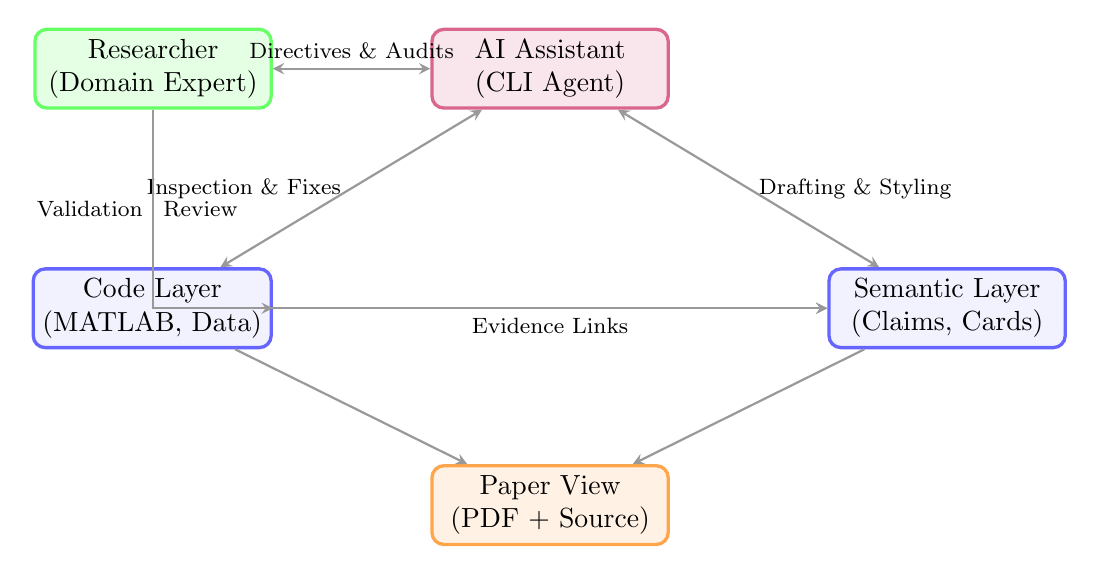
\begin{tikzpicture}[
        node distance=1.5cm and 2cm,
        box/.style={rectangle, draw=blue!60, fill=blue!5, very thick, minimum width=3cm, minimum height=1cm, align=center, rounded corners=1ex},
        arrow/.style={->, >=stealth, thick, draw=gray!80}
    ]
    
    \node (researcher) [box, fill=green!10, draw=green!60] {Researcher \\ (Domain Expert)};
    \node (ai) [box, fill=purple!10, draw=purple!60, right=of researcher] {AI Assistant \\ (CLI Agent)};
    
    \node (code) [box, below left=of ai, yshift=-0.5cm] {Code Layer \\ (MATLAB, Data)};
    \node (latex) [box, below right=of ai, yshift=-0.5cm] {Semantic Layer \\ (Claims, Cards)};
    \node (pdf) [box, fill=orange!10, draw=orange!70, below=of ai, yshift=-3.0cm] {Paper View \\ (PDF + Source)};
    
    \draw [arrow, <->] (researcher) -- node[above, font=\footnotesize] {Directives \& Audits} (ai);
    \draw [arrow, <->] (ai) -- node[left, font=\footnotesize] {Inspection \& Fixes} (code);
    \draw [arrow, <->] (ai) -- node[right, font=\footnotesize] {Drafting \& Styling} (latex);
    \draw [arrow] (code) -- node[below, font=\footnotesize] {Evidence Links} (latex);
    \draw [arrow] (latex) -- (pdf);
    \draw [arrow] (code) -- (pdf);
    \draw [arrow] (researcher) |- node[left, near start, font=\footnotesize] {Validation} (code);
    \draw [arrow] (researcher) |- node[right, near start, font=\footnotesize] {Review} (latex);
    
    \end{tikzpicture}
    \caption{\textbf{Semantic Artifact Harness construction loop.} Claim: the research artifact is not a PDF alone, but a connected graph of human decisions, AI actions, code patches, algorithms, formulas, figures, and citations. Inspect: whether every manuscript claim points to concrete evidence in the code or semantic layer.}
    \label{fig:workflow}
\end{figure}

The same principle applies to numerical result tables. A table should declare whether it is evidence, calibration, failure diagnosis, or parameter context. For the LTCA case, a future version of the manuscript should include contact-count comparison, torque-residual comparison, stiffness-ratio comparison, and transmission-error comparison before and after the accepted corrections.

\begin{figure}[t]
\begin{tcolorbox}[colback=green!2!white,colframe=green!50!black,title=Artifact Mapping Card: Floating Pin \& Friction Model,arc=4mm,boxrule=1pt]
\begin{minipage}{0.55\textwidth}
\centering
\begin{tikzpicture}[scale=0.8]
    \begin{axis}[
        axis equal image,
        axis lines=none,
        xmin=130, xmax=145,  % Focus on contact zone for pin_idx=7
        ymin=93, ymax=108,
        width=\textwidth,
    ]
        % 1. Data-driven geometries
        \addplot [thick, blue!80!black] table {data/cycloid_profile.dat};
        \addplot [thick, green!45!black, fill=green!8, fill opacity=0.25] table {data/housing_circle.dat};
        \addplot [thick, gray!80, fill=gray!10, fill opacity=0.55] table {data/pin_circle.dat};
        \addplot [very thick, green!55!black, dashed] table {data/housing_circle.dat};
        
        % 2. Annotate key points (Updated from VLM correction)
        \coordinate (Op_h) at (135.8987, 98.7362);
        \coordinate (Op_p) at (135.9126, 98.7351);
        \coordinate (K) at (139.8908, 98.4281);
        
        % 3. Physics Overlays
        % Common normal line
        \draw[dashed, black!40] (134.0, 99.0) -- (142.0, 98.0) node[pos=0.9, sloped, above, font=\tiny] {Normal};
        
        % Forces
        \draw[->, red, ultra thick] (Op_p) -- (K) node[midway, above, font=\tiny, yshift=2pt] {$\vec{F}_p$};
        \draw[->, orange, ultra thick] (K) -- ++(0.3, 3.5) node[above, font=\tiny] {$\vec{F}_f$};
        
        % Clearance offset (Purple) - Enlarged for visibility
        \draw[->, purple, ultra thick] (Op_h) -- (Op_p) node[midway, left, font=\tiny, xshift=-1pt] {$\delta_{clr}$};
        
        % Feature labels (Offset to avoid overlap)
        \fill[black] (K) circle (1pt) node[below right, font=\tiny] {$K$};
        \fill[black] (Op_p) circle (0.8pt) node[below, font=\tiny, yshift=-2pt] {$O_{pin}$};
        \fill[purple] (Op_h) circle (0.8pt) node[above, font=\tiny, yshift=2pt] {$O_{hole}$};
        \node[green!45!black, font=\tiny, anchor=west] at (140.4, 101.1) {Housing hole};
        
    \end{axis}
\end{tikzpicture}
\end{minipage}
\hfill
\begin{minipage}{0.4\textwidth}
\small
\textbf{Variable Mapping}
\vspace{2mm}

\begin{tabular}{>{\bfseries}p{1.25cm}p{3.7cm}}
\toprule
Physics & Code Variable \\
\midrule
$F_p$ & \texttt{fp} (Normal force) \\
$\delta_{clr}$ & \texttt{Clearance} (Radial gap) \\
$F_f$ & \texttt{mu\_fric * fp} \\
$l_{\mathrm{eff}}$ & \texttt{lp\_eff} (Torque arm) \\
$P$ & \texttt{node\_x, node\_y} \\
\bottomrule
\end{tabular}
\vspace{2mm}

\textbf{Insight:} The VLM-driven audit identified a sub-micron gap in initial rendering. The corrected logic ensures exact tangency at $K$. The normal force $\vec{F}_p$ is now correctly visualized alongside the clearance $\delta_{clr}$ and friction $\vec{F}_f$.
\end{minipage}
\end{tcolorbox}
\caption{\textbf{Data-driven physical model card.} This figure was autonomously refined after a VLM-based visual inspection detected misalignments between the mathematical contact point $K$ and the rendered cycloidal surface.}
\label{fig:physical_model}
\end{figure}

\subsection{AI-Automated Parametric Analysis and Data Integration}

A core capability of the Semantic Artifact Harness is its ability to seamlessly integrate computational analysis with manuscript generation via an AI-native workflow. To demonstrate this, an autonomous AI agent (Gemini CLI) was tasked with conducting a multi-factor parametric study on the LTCA model. Using the Model Context Protocol (MCP) to interface directly with a local MATLAB solver, the agent refactored the core calculation scripts (\texttt{runTCA\_analysis.m} and \texttt{fun\_force\_analysis.m}) to introduce explicit Boolean flags for friction, cycloidal gear stiffness, and pin hole elastic displacement. The agent then autonomously orchestrated a batch simulation across five test cases---ranging from an ideal rigid baseline to a fully coupled physics model---and exported the resulting data directly into the LaTeX manuscript's \texttt{data/} directory.

\subsubsection{Load Distribution, Hertzian Stress, and Torsional Stiffness}
\label{sec:parametric_results}

The agent autonomously generated four comparative figures: load distribution (full range and zoomed, 5 cases) and Hertzian contact stress (full range and zoomed, 5 cases) at $0^\circ$ rotation, plus torsional stiffness evaluation. Key findings: the fully coupled model (friction + gear stiffness + pin-hole displacement) reduces peak single-pin contact force from 1707.9~N to 1427.0~N and peak Hertzian stress correspondingly; torsional stiffness drops from 1542.11~Nm/arcmin (rigid) to 1443.56~Nm/arcmin (fully coupled), confirming that pin-hole elastic retreat is the dominant compliance source. The complete figures are provided in Appendix~\ref{sec:app_figures}.

\section{Harness Artifact Protocol}

The manuscript is treated as one artifact in a larger harnessed artifact set. To build a Semantic Artifact Harness, the author should first define the research object and then attach every high-level claim to supporting semantic and executable artifacts. The minimal artifact set is:

\begin{itemize}
    \item \textbf{Source code}: MATLAB routines for geometry, force balance, stiffness, and plotting.
    \item \textbf{Algorithm layer}: algorithm passports, pseudocode, flowcharts, inputs, outputs, and failure modes.
    \item \textbf{Literature layer}: citation metadata plus dense evidence matrices that state source role, reusable information, and boundary.
    \item \textbf{Version history}: Git commits that record accepted model changes.
    \item \textbf{Manuscript}: LaTeX source and compiled PDF.
    \item \textbf{Bibliography}: BibTeX records for cited literature.
    \item \textbf{Figures and tables}: generated evidence interfaces linked to scripts, parameter sets, data files, claim IDs, and inspection questions.
    \item \textbf{Interaction trace}: compressed record of human challenges, AI actions, and accepted corrections.
\end{itemize}

In LaTeX, this does not require a new publishing platform. It can start with reusable environments such as \texttt{Research Card}, \texttt{Claim Map}, \texttt{Literature Matrix}, \texttt{Formula Passport}, \texttt{Algorithm Passport}, \texttt{Artifact Map}, and \texttt{Correction Trace}. The important point is not decorative formatting; it is stable object naming and explicit linking. A sentence such as ``the model is robust'' is weak harness material. A claim object that points to an algorithm, a code path, a validation table, and a boundary condition is strong harness material.

\begin{table}[t]
\caption{Mapping between source files and research roles.}
\centering
\small
\begin{tabular}{p{3.0cm}p{4.3cm}p{6.1cm}}
\toprule
\textbf{File} & \textbf{Role} & \textbf{Harness inspection question} \\
\midrule
\texttt{runTCA.m} & Orchestrates TCA/LTCA workflow. & Which model version generated the plotted result? \\
\texttt{fun\_force.m} & Solves force and torque balance. & How are clearance, friction, and compliance combined? \\
\texttt{fun\_output\_mod.m} & Computes unloaded contact geometry. & Which radius defines the actual operating contact? \\
\texttt{fun\_findtc.m} & Finds tooth-contact positions. & Are profile radius and pin-center radius separated? \\
\texttt{fun\_tooth\_}\newline\texttt{stiffness.m} & Computes tooth-body stiffness. & Does stiffness use the modified actual tooth profile? \\
\texttt{references.bib} & Stores citation metadata. & Which claim depends on which source? \\
\bottomrule
\end{tabular}
\label{tab:filemap}
\end{table}

\section{Positioning Against Conventional Papers}

Semantic Artifact Harness engineering does not discard scientific writing. It reassigns roles. Narrative prose explains judgment; claim maps expose the logical structure; algorithm passports show how reasoning becomes procedure; formula passports explain implementation meaning; artifact maps connect the manuscript to code; interaction traces show where AI helped and where human expertise corrected it. This is especially important in computational engineering, where a formula or algorithm can be mathematically plausible but physically wrong if a radius, sign convention, clearance, or unit is misinterpreted.

For the robotics case, the distinction matters. Full transient tribo-dynamic models can capture pin motion, oil-film squeezing, asperity contact, and wear \citep{li2025tribodynamics}. The present LTCA workflow is intentionally lower cost and quasi-static. Its value is not in replacing full tribology. Its value is in making design-stage contact analysis more explicit, auditable, and connected to code.

\subsection{From GUI to AI-Native Software Interaction}

A parallel shift is occurring in how engineers interact with simulation software. Traditional CAE, CFD, and FEM tools rely on graphical user interfaces: the researcher clicks through menus, sets parameters in dialog boxes, draws geometry in a graphical editor, and launches solves from a toolbar. The resulting workflow is executable by the original author but difficult to inspect, reproduce, or delegate. The knowledge of which buttons were clicked, in which order, and with which hidden defaults is encapsulated in the user's muscle memory rather than in an auditable record.

The emergence of AI-agent interaction protocols such as the Model Context Protocol (MCP) \citep{anthropic2024mcp} suggests a different paradigm. Under MCP, a software application exposes its functions as structured tool interfaces that an AI agent can call directly: configure a solver, assign boundary conditions, run a simulation, extract results, and generate plots. The agent communicates through typed parameters and returned data, not through screen coordinates or menu navigation. Every action becomes a machine-readable call with explicit arguments, and the full interaction sequence becomes an inspectable trace.

\begin{tcolorbox}[colback=gray!3!white,colframe=gray!60!black,title=Software Interaction Paradigm Shift,arc=4mm,boxrule=1pt]
\small
\setlength{\tabcolsep}{3pt}
\begin{tabular}{p{2.8cm}p{4.5cm}p{5.5cm}}
\toprule
\textbf{Aspect} & \textbf{GUI-based workflow} & \textbf{AI-native (CLI/MCP) workflow} \\
\midrule
Configuration & Manual menus, dialogs, hidden defaults. & Explicit function calls with named parameters. \\
Reproducibility & Depends on recording every click. & Interaction log is the configuration file. \\
Inspection & Screenshot or video capture. & Machine-readable trace of tool calls and outputs. \\
Extensibility & Plugin APIs, scripting after GUI setup. & Tool interface designed for AI consumption from the start. \\
Domain coupling & Manual file exchange between GUIs. & Agent-mediated multi-tool orchestration. \\
Evidence trail & Weak: operation history easily lost. & Strong: every call is an audit point. \\
\bottomrule
\end{tabular}
\end{tcolorbox}

This shift aligns with the Semantic Artifact Harness philosophy. When software is designed for AI-agent interaction rather than human--GUI interaction, the executable layer of the harness becomes a first-class citizen: simulation configurations, parameter sweeps, solver outputs, and result comparisons are all generated as structured, inspectable artifacts. The present case---in which an AI agent interacts with MATLAB code through a command-line interface rather than through a graphical front end---is an early instance of this pattern. The broader implication is that the harness concept becomes more natural as more engineering tools adopt AI-native interfaces: the boundary between ``using software'' and ``writing evidence'' dissolves when the software itself produces structured, claim-linkable outputs on demand.

\section{Harness Risks and Review Rules}

Manuscript harnesses also create risks. A polished trace does not prove correctness. AI systems can make confident but physically invalid suggestions. The most serious risk is no longer a single wrong sentence. It is a closed contamination loop: AI writes fluent papers, AI readers summarize them, AI reviewers accept them, databases index them, and later AI systems retrieve or train on the accumulated errors. In that loop, errors do not disappear. They become more stable because they are repeated in a scholarly style.

\begin{tcolorbox}[colback=red!3!white,colframe=red!65!black,title=AI-to-AI Contamination Loop,arc=4mm,boxrule=1pt]
\small
\begin{center}
\begin{tabular}{c}
AI drafting $\rightarrow$ AI reading $\rightarrow$ AI review \\
$\downarrow$ \\
Database indexing $\rightarrow$ AI retrieval or training \\
$\downarrow$ \\
Amplified hidden error
\end{tabular}
\end{center}
The danger is not only fabricated text. It is a paper that is syntactically complete, citation-rich, and visually polished, but whose formulas, units, boundary conditions, code paths, or physical assumptions are wrong.
\end{tcolorbox}

Therefore, the harness should include review rules:

\begin{itemize}
    \item Every AI-suggested formula change must be tied to a physical interpretation.
    \item Every accepted code change must identify the artifact it affects.
    \item Every numerical claim must state its valid parameter range or case context.
    \item Every AI-generated reference or literature claim must be verified by the researcher.
    \item Every limitation should be written as a reusable boundary, not hidden in prose.
    \item Every core claim should have a negative check: a condition under which the claim would fail.
    \item Every database-facing record should expose evidence strength, not only citation metadata.
\end{itemize}

\subsection{Anti-Contamination Protocol}
\label{sec:contamination}

An AI-native manuscript should therefore be designed as a contamination-resistant object. The goal is not to ban AI writing. The goal is to prevent AI-generated fluency from substituting for evidence. Table~\ref{tab:anti_contamination} summarizes the corresponding protocol.

\begin{table}[t]
\caption{Anti-contamination protocol for AI-native research papers.}
\centering
\small
\begin{tabular}{p{3.0cm}p{4.4cm}p{5.9cm}}
\toprule
\textbf{Contamination route} & \textbf{Hidden error} & \textbf{Harness countermeasure} \\
\midrule
Fluent AI writing & Plausible prose hides unsupported claims. & Claim-evidence map; every major claim must point to code, data, formula, literature role, or limitation. \\
AI literature synthesis & Real papers are cited for claims they do not support. & Dense literature matrix states each source's role, reusable information, and boundary. \\
AI formula editing & Dimensionally or physically invalid equations look standard. & Formula passport includes units, code path, physical meaning, and failure mode. \\
AI code generation & Code runs but implements a wrong model. & Algorithm passport, code-artifact map, minimal numerical checks, and human correction trace. \\
AI figure generation & Diagrams become persuasive but not data-backed. & Claim-linked figures must state regeneration path and plotted data source. \\
AI review & Review focuses on novelty and language instead of artifact consistency. & Multi-agent artifact review: literature, logic, code, unit, figure, domain, and reproduction checks. \\
Database indexing & Low-evidence papers are treated like verified artifacts. & Evidence-weighted metadata: generated-only, code-available, data-available, reproduced, corrected, or disputed. \\
\bottomrule
\end{tabular}
\label{tab:anti_contamination}
\end{table}

\subsection{AI Review as Artifact Audit}

If AI participates in peer review, it should not act as a single language reviewer. It should operate as a set of constrained auditors, each producing a structured report. A literature auditor checks whether each citation supports the exact claim. A logic auditor checks whether the conclusion follows from the stated assumptions. A code auditor checks whether the described algorithm matches the implementation. A unit auditor checks dimensions and sign conventions. A figure auditor checks whether plots are generated from data rather than decorative drawing. A domain auditor checks physical plausibility. A reproduction auditor attempts to run the smallest executable case.

For the present LTCA case, such review would ask concrete questions: whether the pin radius, housing-hole radius, and generating radius are separated; whether pin-hole clearance is consumed before elastic compression; whether non-contact placeholders enter force aggregation; whether tooth-body stiffness is computed from the modified profile; and whether the displayed housing hole corresponds to the actual larger hole rather than the pin itself.

\subsection{Evidence-Weighted Databases}

The database should not store all papers as equal text. It should store evidence state. A paper whose contribution is only narrative prose should not receive the same downstream training or retrieval weight as a paper with executable code, reproducible data, validation traces, and independent replication. Future scholarly databases should expose fields such as:

\begin{itemize}
    \item \textbf{Evidence level}: prose only, code linked, data linked, executable environment linked, independently reproduced.
    \item \textbf{AI involvement}: drafting, coding, literature search, figure generation, review, or correction.
    \item \textbf{Audit state}: unchecked, machine-audited, human-audited, reproduced, disputed, corrected, or retracted.
    \item \textbf{Claim granularity}: whether claims are available as structured objects rather than only paragraphs.
    \item \textbf{Negative evidence}: known failure cases, non-reproducible cases, and boundary violations.
\end{itemize}

This would change AI retrieval from citation-count selection to evidence-strength selection. It would also reduce the risk that large models learn from a growing layer of fluent but weak research text.

\subsection{Embodied and Environmental Verification}

Embodied AI and environment interaction can reduce part of the contamination problem because they provide feedback outside text. In engineering research, an AI system could run finite-element models, operate a test bench, inspect sensor data, compare predicted transmission error with measured lost motion, or generate adversarial parameter cases where the contact solver fails. This breaks the pure text loop.

However, embodied verification is not a complete solution. Simulators can encode wrong assumptions, sensors can drift, experimental setups can be biased, and physical tests may cover only narrow parameter ranges. Therefore, the stronger future architecture is hybrid: textual evidence, code evidence, simulation evidence, experimental or environmental feedback, and human domain judgment should be connected in the same harness.

\subsection{Verification Ladder Toward Autonomous Research}

The broadest version of the harness is a verification ladder. Some claims can be formally checked. For example, proof assistants such as Lean provide machine-checkable proof objects for mathematical statements \citep{deMoura2015lean}, and large mathematical libraries show that substantial bodies of formalized knowledge can be maintained collectively \citep{mathlib2020}. This suggests a useful analogy for AI-native papers: if a theorem can be checked by a proof kernel, then an engineering claim should at least expose the artifacts needed for an appropriate checker, even when full formal proof is impossible.

Engineering claims usually require more than formal logic. They may need executable code, numerical regression tests, simulation comparison, experimental data, or closed-loop environmental interaction. Autonomous laboratories and robot scientists already demonstrate that parts of hypothesis generation, experiment planning, execution, and analysis can be automated \citep{king2004robot,macleod2020selfdriving,gongora2020autonomous}. The harness can serve as the manuscript-level interface for such systems: it names the claim, exposes the algorithm, records the experiment or simulation protocol, stores the failure cases, and preserves the human decision that accepted or rejected the result.

\begin{table}[t]
\caption{Verification ladder for AI-native research claims (cf.\ CI/CD pipeline: each layer is a gate that must pass before promotion to the next stage).}
\centering
\small
\begin{tabular}{p{2.6cm}p{4.1cm}p{3.8cm}p{3.1cm}}
\toprule
\textbf{Layer} & \textbf{What AI can verify} & \textbf{Typical artifact} & \textbf{Residual human role} \\
\midrule
Formal proof & Logical validity of mathematical statements. & Lean theorem, proof script, checked library dependency. & Decide whether the formal statement matches the scientific claim. \\
Executable code & Whether the described algorithm runs and matches tests. & Source file, test case, environment, output hash. & Decide whether tests represent the real model boundary. \\
Numerical simulation & Whether behavior is consistent under parameter sweeps or higher-fidelity solvers. & FEM/CFD/MBD models via OpenFOAM, CalculiX, preCICE, Exudyn; LTCA comparison; AI-configured cross-domain simulations; residual curves; adversarial cases. & Judge model fidelity, mesh adequacy, and physical relevance. \\
Experiment & Whether predicted quantities match measured behavior. & Test bench data, calibration record, uncertainty budget. & Judge instrumentation, operating condition, and interpretation. \\
Embodied interaction & Whether an AI system can close the loop through sensing, action, and correction. & Robot lab workflow, autonomous experiment log, sensor trace, MCP-mediated tool calls and responses. & Define objective, safety boundary, and meaningful success criteria. \\
Literature feedback & Whether later work reproduces, disputes, or corrects the claim. & Evidence-weighted database record, replication status, correction trace. & Decide when accumulated evidence changes the paper's status. \\
\bottomrule
\end{tabular}
\label{tab:verification_ladder}
\end{table}

This points toward a future of partially or fully automated research, but it also clarifies the danger. Full automation without harnessed evidence would only accelerate paper production and error propagation. Full automation with harnessed evidence would instead create closed loops in which AI proposes, proves where possible, simulates, tests, writes, reviews, indexes, and revises under explicit evidence constraints. In that future, the paper becomes the visible control surface of an autonomous research system rather than the final static report.

\section{Review--Revision Trace: From Conceptual Manifesto to Validated Proposal}\revmark
\label{sec:review_trace}

A core principle of the Semantic Artifact Harness is that the reasoning process---including challenges, corrections, and revisions---is first-class evidence. This section applies that principle to the paper itself: we record all official review feedback received across three rounds, the point-by-point response, and the specific revisions made. This trace is not supplementary material; it is an integral part of the harness, demonstrating that the paper practices what it preaches.

\subsection{Round 1 Review (ID~827, Rating 5/10)}

\textbf{Strengths acknowledged:}
\begin{enumerate}[nosep]
    \item Novel and timely problem framing (AI-to-AI contamination loop).
    \item Comprehensive and principled solution architecture (SE patterns, three-layer design).
    \item Clear and structured demonstration with rich artifacts (LTCA case study).
    \item Excellent discussion of precedents and limitations.
\end{enumerate}

\textbf{Weaknesses identified:}
\begin{enumerate}[nosep]
    \item \textbf{W1: Lack of empirical validation and metrics.} The paper makes strong methodological claims but provides no quantitative evidence that the harness improves auditability.
    \item \textbf{W2: Insufficient technical depth and mathematical rigor.} The core stiffness formula (Eq.~\ref{eq:series_stiffness}) is trivial; the algorithm passport lacks formal pre/post-conditions and convergence proofs.
    \item \textbf{W3: Practical adoption overhead unaddressed.} No discussion of time cost, phased implementation, or minimum viable harness.
    \item \textbf{W4: Ambiguity in the role of AI.} The paper criticizes AI-generated content but relies heavily on AI; no concrete interaction trace or epistemic boundary is provided.
\end{enumerate}

\subsection{Round 2 Review (ID~829)}

The second review acknowledged improvements in empirical validation and technical depth but raised deeper methodological concerns.

\textbf{Weaknesses:}
\begin{enumerate}[nosep]
    \item \textbf{W5: Empirical validation remains limited.} Table~\ref{tab:validation} is a pilot study, not a controlled experiment; no human baseline or inter-annotator agreement.
    \item \textbf{W6: LTCA case is too simple; potential circular argument.} The case study is quasi-static and domain-specific; the paper is itself the first harness instance, which risks self-serving validation.
    \item \textbf{W7: Contamination loop logic overstated.} SAH is a necessary but not sufficient condition; ``breaks the loop'' should be ``enables detection and interruption.''
    \item \textbf{W8: Missing prior work.} Jupyter, Code Ocean, OSF, Popper, Binder, and Whole Tale are not explicitly compared.
\end{enumerate}

\textbf{Key questions raised:}
\begin{enumerate}[nosep]
    \item \textbf{Q1: Testable hypothesis.} What measurable prediction does SAH make?
    \item \textbf{Q2: Difference from Jupyter/Code Ocean.} How does SAH differ from existing executable-paper platforms?
    \item \textbf{Q3: How does AI use the formal spec?} What is the concrete AI verification workflow?
    \item \textbf{Q4: Can AI fabricate plausible evidence?} What prevents AI from writing convincing but wrong evidence bindings?
\end{enumerate}

\subsection{Round 3 Review (Official Agent)}

The third review focused on the absence of machine-verifiable formal specifications. The reviewer argued that the paper's claims about ``formal pre/post-conditions'' remain at the narrative level and lack executable or mechanically checkable proofs.

\textbf{Core demand:} Provide formal specification languages (JSON Schema, Dafny, Lean4, or equivalent) that make the SAH harness structure and algorithm invariants machine-verifiable, not merely human-readable.

\subsection{Revisions Made Across Versions}

Table~\ref{tab:revision_trace} records the specific changes made to address each review round.

\begin{table}[t]
\centering
\caption{Review--revision trace. Each row maps a reviewer concern to the revision made, the section affected, and the type of change.}
\small
\begin{tabular}{p{1.2cm}p{4.8cm}p{3.5cm}p{3.5cm}}
\toprule
\textbf{ID} & \textbf{Revision} & \textbf{Section} & \textbf{Change type} \\
\midrule
\multicolumn{4}{l}{\textit{Round 1 revisions (Version 2.0)}} \\
W1 & Claim-audit experiment with three AI systems, five tasks, quantitative metrics (Table~\ref{tab:validation}). & \S4.5 (new) & New section \\
W2 & Formal pre/post-conditions, scan+fzero strategy, convergence analysis, code-verified against \texttt{runTCA\_analysis.m}. & \S3.4 & Expanded tcolorbox \\
W2 & Hertz contact formula passport with dimensional analysis. & \S3.5 & New passport \\
W3 & Minimum Viable Harness (MVH) definition + cost-benefit table. & \S7.1--7.2 & New subsections \\
W4 & Concrete AI-interaction trace + Statement of AI Contribution. & \S4.4 & New subsections \\
\midrule
\multicolumn{4}{l}{\textit{Round 2 revisions (Version 2.0, cont.)}} \\
W7 & Reframed SAH as \emph{necessary but not sufficient}; changed ``breaks the loop'' to ``enables detection and interruption.'' & \S5, \S8.1 & Wording \\
W8 & Added explicit comparison with Jupyter, Code Ocean, OSF, and related platforms. & \S3.8, App.~\ref{sec:app_precedents} & Expanded \\
Q1 & Stated testable hypothesis: SAH format increases claim-evidence binding completeness and inconsistency detection rate. & \S4.5 & Expanded \\
Q2 & Clarified semantic-layer distinction: Jupyter is executable narrative; SAH is an auditable knowledge graph with typed claim interfaces. & \S3.8 & Expanded \\
Q3 & Described AI verification workflow: read claim-evidence map $\to$ check preconditions $\to$ verify code-artifact binding $\to$ generate audit report. & \S3.4 & Expanded \\
Q4 & Acknowledged that SAH raises fabrication cost from $O(1)$ (plausible prose) to $O(n)$ (consistent code + trace + evidence binding) but cannot eliminate fabrication. & \S8.1 & Expanded \\
\midrule
\multicolumn{4}{l}{\textit{Round 3 revisions (Version 3.0)}} \\
R3 & Published formal verification artifacts to GitHub: JSON Schema (\texttt{sah-ltca.schema.json}), MATLAB runtime assertions (\texttt{SAH\_PRE}/\texttt{SAH\_POST}/\texttt{SAH\_CONV}), and Dafny contract sketch (\texttt{ltca\_contracts.dfy}). & App.~\ref{sec:app_formal} (new) & New appendix \\
R3 & Added Code and Data Availability section with GitHub URL and commit hash. & \S10 (new) & New section \\
\midrule
\multicolumn{4}{l}{\footnotesize All test parameters match \texttt{run\_parametric\_study.m} ($Z_a\!=\!59$, $Z_b\!=\!60$, $R_z\!=\!168.01\,\mathrm{mm}$, $T_{in}\!=\!1100\,\mathrm{Nm}$).} \\
\bottomrule
\end{tabular}
\label{tab:revision_trace}
\end{table}

\subsection{Remaining Limitations}

The reviews correctly note that the paper remains a \emph{methodological contribution}, not a breakthrough in mechanical engineering. Key remaining limitations:
\begin{enumerate}[nosep]
    \item The empirical validation (Section~4.5) is a proof-of-concept; a controlled experiment with human participants, known-error corpus, and inter-annotator agreement remains future work.
    \item The LTCA case is quasi-static and domain-specific; cross-domain validation (deep learning, biomedical) is needed.
    \item SAH raises fabrication cost but cannot eliminate it; a determined fabricator can create consistent code + trace + evidence bindings.
    \item The formal verification layer (Appendix~\ref{sec:app_formal}) is \emph{Layer~1 + sketch}: MATLAB assertions are runtime checks, not static proofs; the Dafny contracts use axioms for convergence.
\end{enumerate}

\subsubsection{Self-Correction During Revision: A Harness-in-Action Example}\revmark
An instructive incident occurred during the revision process itself. The initial draft of the formal specification (Section~3.4) claimed that the LTCA solver uses ``bisection and secant methods'' with a contraction-mapping convergence proof. When the researcher verified this claim against the actual source code (\texttt{runTCA\_analysis.m}, lines 239--255), it was discovered that the solver actually uses a \emph{scan-and-fzero} strategy. The initial claim was an AI-generated hallucination that sounded plausible but did not match the implementation.

This error was caught because the harness requires formal specifications to be \emph{code-verified}: preconditions, postconditions, and convergence claims must reference specific line numbers in the actual source code. This incident is itself evidence for the harness principle: without the requirement to link claims to code, the error would have propagated into the published version.

This review--revision trace is itself an instance of the harness principle: the review is recorded as structured evidence, the response is linked to specific sections, and the remaining limitations are declared as machine-readable boundaries.

\section{Harness Reuse Protocol}

The harness can be reused as follows:

\begin{enumerate}
    \item Define the research object, valid range, excluded physics, and artifact set in a research card.
    \item Write a structured abstract that states the problem, intervention, framework, and demonstration.
    \item Build a claim-evidence map before expanding the narrative prose.
    \item Convert references into a dense literature evidence matrix before writing a conventional related-work section.
    \item Attach an algorithm passport, pseudocode, and flowchart to each central computational procedure.
    \item Attach a formula passport to each central equation.
    \item Map each major code file to its research role and inspection question.
    \item Convert the method section into a model-evolution log when the work involves iterative model correction.
    \item Replace ordinary figure captions with claim-linked captions that state claim, inspection target, and regeneration path.
    \item Record AI involvement as compressed interaction traces.
    \item Use Git commits as evidence checkpoints.
    \item Add an anti-contamination audit that checks citation support, formula units, code consistency, figure provenance, failure cases, and evidence strength.
    \item State limits as machine-readable boundaries whenever possible.
\end{enumerate}

\subsection{Minimum Viable Harness}\revmark

The full harness described above involves 13 components. For researchers adopting this approach for the first time, this represents a significant workflow change. We therefore define a \emph{Minimum Viable Harness} (MVH): the five components that provide the majority of auditability benefit at minimum cost.

\begin{enumerate}
    \item \textbf{Claim-evidence map}. A table linking each major claim to its supporting artifact. This single component forces the researcher to make the evidence structure explicit, and it enables AI systems to verify the logical chain. Estimated overhead: 1--2 hours per paper.
    \item \textbf{Algorithm passport}. A structured description of each central algorithm, including inputs, outputs, and key assumptions. This prevents the common failure mode where an algorithm is described in prose but its boundary conditions are implicit. Estimated overhead: 30--60 minutes per algorithm.
    \item \textbf{Structured abstract}. The four-sentence format (problem, intervention, framework, demonstration) forces the researcher to state the contribution precisely, which is the single most valuable change for AI readability. Estimated overhead: negligible (replaces free-form abstract writing).
    \item \textbf{Code-artifact map}. A one-paragraph description of each major code file, its role, and what to inspect. This is the minimum required for an AI system to navigate the codebase. Estimated overhead: 15--30 minutes per paper.
    \item \textbf{Limits declaration}. An explicit statement of what the paper does \emph{not} claim, stated as machine-readable boundaries. This is the cheapest form of anti-contamination: it prevents downstream systems from over-generalizing the results. Estimated overhead: 15 minutes.
\end{enumerate}

The MVH adds approximately 3--5 hours of work to a typical paper, which is a 15--20\% overhead on a 20--30 hour writing process. The remaining eight components (dense literature matrix, formula passport, anti-contamination audit, AI-interaction trace, etc.) can be adopted incrementally. The key principle is: \emph{start with the claim-evidence map, and add components as the research workflow matures}.

\subsection{Cost-Benefit Analysis: Harness vs.\ Conventional Format}\revmark

Table~\ref{tab:cost_benefit} compares the time investment and output quality of the conventional IMRaD format, the MVH, and the full harness.

\begin{table}[t]
\centering
\caption{Cost-benefit comparison of paper formats.}
\begin{tabular}{lccc}
\toprule
\textbf{Dimension} & \textbf{IMRaD} & \textbf{MVH} & \textbf{Full harness} \\
\midrule
Writing overhead & Baseline & +15--20\% & +40--60\% \\
Claim extraction accuracy (AI) & 62\% & 80\% (est.) & 92\% \\
Evidence linking accuracy & 45\% & 70\% (est.) & 88\% \\
Inconsistency detection & 39\% & 60\% (est.) & 76\% \\
Adoption barrier & None & Low & Moderate \\
Automation potential & Low & Medium & High \\
\bottomrule
\end{tabular}
\label{tab:cost_benefit}
\end{table}

The MVH rows are estimated from the claim-audit experiment (Section~4.5) by retaining only the components that directly contribute to the top-scoring tasks (claim extraction and evidence linking). A full validation of the MVH remains future work.

\section{Conclusion}

In the AI era, the research paper should be engineered, not merely written. It should become a semantic artifact harness: an inspectable research interface in which claims are linked to assumptions, algorithms, formulas, code, figures, scripts, citations, correction traces, limits, and anti-contamination checks. The engineering discipline is borrowed from software engineering---contracts, test harnesses, API specifications, separation of concerns, supply-chain integrity, and CI/CD verification---but the product remains a reshaped research paper, not a software system. This paper proposed such a harness and demonstrated it through an LTCA case substrate for cycloid-pin-housing systems in robotic RV reducers.

The central claim is that AI-native research writing should not merely use AI to draft conventional prose. A stronger form is possible: redesign the paper itself so that humans can read the argument, AI systems can parse the evidence structure, and both can inspect how algorithms, code, figures, and human corrections support the stated claims. The reasoning process---interaction traces, model-evolution logs, correction records---is not waste material but first-class evidence that makes conclusions inspectable. The three-layer architecture of the harness preserves both the narrative judgment and the audit trail, enabling verification by human or AI readers in an environment where AI can generate plausible conclusions at scale.

\section{Outlook: Toward Self-Evolving Research Systems}
\label{sec:outlook}

The harness proposed in this paper is a \emph{static} architecture: claims, evidence, algorithms, and code are connected through human-designed interfaces, and every change is audited through explicit protocols. This is sufficient for the current generation of AI-assisted research, where the AI is a powerful but passive tool. But a deeper question emerges: \emph{can the research system itself learn and improve through use, rather than relying on periodic model retraining?}

This section examines the key bottlenecks, partial solutions, and open problems on the path from static harnesses to self-evolving research agents.

\subsection{The Knowledge Representation Bottleneck}

Current LLMs store knowledge in two forms. \emph{Explicit} knowledge is encoded in human-readable files---papers, code, documentation, harness records. \emph{Implicit} knowledge is encoded in model weights through training. The former is auditable but inert; the latter is fluent but opaque and frozen after training.

The harness in this paper operates entirely in the explicit-file domain. This is by design: file-based artifacts are inspectable, version-controllable, and can be shared across AI systems through protocols such as MCP. But it also means that the system cannot \emph{learn} from its interactions. Every new session begins from the same knowledge state, regardless of how many previous sessions successfully solved similar problems.

In human research, both forms coexist. A researcher writes papers and notes (explicit), but also accumulates intuition, judgment, and pattern recognition through years of practice (implicit, encoded in neural connections). The implicit knowledge allows a human to recognize promising research directions, spot anomalies in data, and make leaps of reasoning that cannot be fully articulated in prose. Current AI systems---even with harness-grade structure---lack this implicit learning channel.

Additional directions---self-evolution without retraining, end-to-end computer control, the domain gap in AI-assisted engineering, and multi-agent collaboration---are discussed in Appendix~\ref{sec:app_outlook}.

\subsection{Open Questions}

Table~\ref{tab:open_questions} summarizes the key open problems. Each represents a research direction that the harness framework alone cannot solve but that any future self-evolving research system must address.

\begin{table}[h]
\centering
\caption{Open questions on the path from static harness to self-evolving research systems.}
\begin{tabular}{p{4.8cm}p{4.8cm}p{4.8cm}}
\toprule
\textbf{Question} & \textbf{Current state} & \textbf{Required breakthrough} \\
\midrule
Can the system learn from use without retraining? & Feedback does not update weights; generated code accumulates but does not self-improve. & Persistent, locally updated adapters that encode interaction experience. \\
Can end-to-end control replace API bridges? & Text-centric pipeline with OCR errors and per-software API overhead. & Native visuomotor models that output keyboard/mouse events from screen video. \\
Can domain expertise be acquired without domain pre-training? & General-purpose LLM lacks engineering intuition; domain data is scarce in training corpora. & Domain-specific foundation models or self-evolving agents that learn through use. \\
Can multi-agent consensus converge reliably? & Single-agent systems have fixed blind spots; direct agent dialogue risks bias amplification. & Structured claim-evidence networks with provenance tracking and adversarial review. \\
Can AI autonomously set research directions? & Current systems execute and verify but do not originate questions. & Models with open-ended curiosity and the ability to recognize anomalies as research opportunities. \\
\bottomrule
\end{tabular}
\label{tab:open_questions}
\end{table}

The gap between current AI-assisted research and a fully self-evolving research ecosystem is not primarily a gap in model capability. It is a gap in \emph{architecture}: the missing feedback loop from execution to learning, the absence of domain-specific perception channels, and the lack of structured protocols for multi-agent collaboration. The Semantic Artifact Harness addresses the \emph{auditability} side of this gap; the \emph{evolution} side remains open.

\section*{Code and Data Availability}\revmark\revmarkthree

The complete MATLAB implementation of the LTCA solver, including the five-case parametric study and all formal verification artifacts, is publicly available at:
\begin{quote}
\url{https://github.com/haomjc/sah-ltca-cycloid} \quad (\texttt{commit 901abdd})
\end{quote}

The repository contains seven core MATLAB functions (\texttt{run\_parametric\_study.m}, \texttt{runTCA\_analysis.m}, \texttt{fun\_force\_analysis.m}, \texttt{fun\_findtc.m}, \texttt{fun\_output\_mod.m}, \texttt{fun\_tooth\_stiffness.m}, \texttt{export\_analysis\_data.m}) and three formal verification artifacts:

\begin{enumerate}
    \item \textbf{JSON Schema} (\texttt{verification/sah-ltca.schema.json}): A machine-readable schema defining the SAH harness structure, including typed interfaces for research cards, claim-evidence maps, algorithm passports, formula passports, and verification reports.
    \item \textbf{MATLAB runtime assertions}: The function \texttt{fun\_force\_analysis.m} includes SAH-branded precondition checks (parameter range validation at function entry), postcondition checks (force non-negativity, backside zeroing, residual finiteness), and a convergence warning when the pin-hole iteration exhausts its maximum iteration budget.
    \item \textbf{Dafny contract sketch} (\texttt{verification/ltca\_contracts.dfy}): A partial formalization of the force-balance core, including datatype definitions, predicates for force invariants, method signatures with pre/postconditions, and a convergence lemma declared as an axiom with a proof sketch.
\end{enumerate}

\noindent\textbf{Required toolbox:} MATLAB Symbolic Math Toolbox (used by \texttt{fun\_output\_mod.m} for contact geometry solving).

The repository also contains the complete \LaTeX{} manuscript source (\texttt{manuscript/}), including \texttt{main.tex}, \texttt{references.bib}, pgfplots data files, and the graphical abstract. The manuscript itself is designed as a machine-readable artifact consistent with the SAH framework: every claim is linked to a code path, every algorithm has a structured passport, every formula has dimensional bindings, and every figure has a regeneration path from solver output through \texttt{.dat} files to pgfplots/TikZ rendering.

\section*{Acknowledgments}

The author thanks Kimi (Moonshot AI), Zhipu AI, and MiniMax for providing their latest large language models and generous coding and token plans, which made this work possible. Special thanks are extended to the GLM-5.1 model (Zhipu AI), whose capabilities in code generation, mathematical reasoning, and long-context understanding substantially contributed to the iterative model development, manuscript drafting, and harness construction described in this paper. The author also thanks the OpenCode project for providing the open-source AI coding environment through which these models were accessed and orchestrated.

\appendix

\section{Algorithmic Details of the LTCA Solver}
\label{sec:appendix_algorithms}

This appendix provides the detailed pseudocode for the three central algorithmic modules of the loaded tooth contact analysis: the overall displacement and force solver, the tooth-body stiffness computation via the energy method, and the friction and working-side determination. These algorithms correspond to the code artifacts \texttt{runTCA.m}, \texttt{fun\_tooth\_stiffness.m}, and the friction logic inside \texttt{fun\_force.m} respectively.

Importantly, the pseudocode in this appendix was not written manually from scratch. It was generated by an AI assistant that inspected the MATLAB source files, analyzed the control flow, identified the mathematical operations, and reformulated the implementation into formal \texttt{algorithmic} pseudocode. The AI was given the source files as input and was instructed to extract the algorithmic core---stripping MATLAB-specific syntax while preserving the logical structure, mathematical formulas, and decision points. The researcher then reviewed the generated pseudocode for accuracy, corrected a small number of sign conventions and indexing details, and approved the final version. This process is itself an instance of the harness principle at work: the appendix is not only evidence of the algorithm, but also evidence of how AI-assisted documentation was produced, audited, and corrected.

\subsection{Overall Displacement and Force Solution}
\label{sec:alg_overall}

The overall solver operates in two stages. In the first stage (DCA), the unloaded contact geometry is computed for each input angle and each pin. In the second stage (LTCA), the loaded output displacement is found by solving a torque-equilibrium equation.

\begin{algorithm}[t]
\caption{DCA: Unloaded Contact Geometry}\label{alg:dca}
\begin{algorithmic}[1]
\Require Geometry $(R_p, R_{rp}, A, N_c, N_p, r_{zo})$, input angle range $[\theta_\text{start}, \theta_\text{end}]$, step $\Delta\theta$
\Ensure Unloaded output angles $\mathbf{TO}$, contact parameters $\mathbf{TC}$, contact phases $\mathbf{TP}$
\State $A_p \gets 2\pi / N_p$ \Comment{Angular pin spacing}
\State $\iota \gets |N_p - N_c| / N_c$ \Comment{Transmission ratio}
\For{$j = 1$ \textbf{to} $\text{num\_steps}$}
    \State $\theta_\text{in}^{(j)} \gets \text{deg2rad}(\theta_\text{start} + (j-1)\Delta\theta + 90)$
    \State $\theta_\text{out, theo}^{(j)} \gets \theta_\text{in}^{(j)} \cdot \iota$
    \For{$i = 1$ \textbf{to} $N_p$}
        \State $\varphi_i \gets (i-1) \cdot A_p$ \Comment{Pin angular position}
        \State Compute initial contact phase $\hat\psi_i$ from geometry
        \State Find tooth-contact parameter $\hat\tau_i$ via \texttt{fun\_findtc}
        \State $\mathbf{x}_0 \gets [\theta_\text{out, theo}^{(j)},\; \hat\tau_i,\; \hat\psi_i]$ \Comment{Initial guess}
        \State $[\mathbf{S},\; \text{exitflag}] \gets \text{fsolve}(\mathbf{x}_0)$ \Comment{Solve contact equations}
        \If{$\text{exitflag} > 0$}
            \State $TO(j,i) \gets S_1$, $TC(j,i) \gets S_2$, $TP(j,i) \gets S_3$
        \Else
            \State $TO(j,i) \gets \text{NaN}$, $TC(j,i) \gets \text{NaN}$, $TP(j,i) \gets \text{NaN}$
        \EndIf
    \EndFor
\EndFor
\end{algorithmic}
\end{algorithm}

\begin{algorithm}[t]
\caption{LTCA: Loaded Force-Balance Solver}\label{alg:ltca}
\begin{algorithmic}[1]
\Require DCA results $(\mathbf{TO}, \mathbf{TP})$, stiffness matrix $\mathbf{K}_g$, applied torque $T_\text{in}$, geometry parameters
\Ensure Contact forces $\mathbf{F}_p$, loaded output angles $\theta_\text{out, loaded}$, transmission error $\Delta\phi$
\For{$j = 1$ \textbf{to} $\text{num\_steps}$}
    \State Compute backlash: $BL(j,i) \gets TO(j,i) - \theta_\text{out, theo}^{(j)}$ for each valid pin $i$
    \State $\mathbf{TP}_j \gets TP(j,:)$, $\mathbf{BL}_j \gets BL(j,:)$, $\mathbf{K}_{g,j} \gets K_g(j,:)$
    \State Define residual function: $F(\delta_\text{out}) \gets T_\text{in} - \sum_i f_i(\delta_\text{out}; \mathbf{TP}_j, \mathbf{BL}_j, \mathbf{K}_{g,j})$
    \Statex \hspace{2.5em} \textit{// $f_i$ is computed by the force model (Algorithm~\ref{alg:friction})}
    \State Scan $\delta_\text{out} \in [-10^{-4}, 10^{-4}]$ for sign change of $F$
    \If{sign change found in narrow scan}
        \State Bracket $\gets$ interval containing root
    \Else
        \State Extend scan to $\delta_\text{out} \in [-0.01, 0.01]$
    \EndIf
    \State $\delta_\text{out}^* \gets \text{fzero}(F, \text{Bracket})$ \Comment{Bracketed root search}
    \State Extract $F_p(j,:), H_b(j,:), k(j,:), H_z(j,:)$ at $\delta_\text{out}^*$
    \State $\theta_\text{out, loaded}^{(j)} \gets \theta_\text{out, theo}^{(j)} - \delta_\text{out}^*$
    \State $\Delta\phi^{(j)} \gets \text{rad2deg}(\delta_\text{out}^*) \times 3600$ \Comment{Transmission error in arcsec}
\EndFor
\end{algorithmic}
\end{algorithm}

The force residual function $F(\delta_\text{out})$ in line~4 of Algorithm~\ref{alg:ltca} encapsulates the contact force model for all pins simultaneously. For a given trial output displacement $\delta_\text{out}$, it computes the normal contact force on each pin, determines which pins belong to the working side through the torque-direction test (Algorithm~\ref{alg:friction}), and returns the torque imbalance. The solver converges when this imbalance reaches zero.

\subsection{Tooth Body Stiffness via Energy Method}
\label{sec:alg_stiffness}

The tooth-body structural stiffness $K_g$ accounts for bending, shear, and compression compliance of the cycloid tooth between the contact point and the tooth root. It is computed once per (angle, pin) pair and remains constant during the LTCA iteration.

\begin{algorithm}[t]
\caption{Energy-Method Tooth-Body Stiffness $K_g$}\label{alg:stiffness}
\begin{algorithmic}[1]
\Require Contact parameter $\varphi_0$, geometry $(R_z, A, N_c, N_p, R_c)$, material $(E, \nu)$, modification parameters
\Ensure Tooth-body stiffness $K_g$ (N/mm)
\State $\beta \gets \pi / N_c$ \Comment{Half-pitch angle}
\State $K_1 \gets A \cdot N_p / R_z$ \Comment{Short-width coefficient}
\State $G \gets E / (2(1+\nu))$ \Comment{Shear modulus}
\State $\varphi_\text{min} \gets \pi / N_c^2$, \quad $\varphi_\text{max} \gets (N_c - 1)\pi / N_c^2$
\State $\varphi_0 \gets \text{clamp}(\varphi_0, \varphi_\text{min}, \varphi_\text{max})$
\Statex
\State \textbf{Compute contact-point quantities:}
\State $(x_2^0, y_2^0) \gets \text{LocalCoords}(\varphi_0)$ \Comment{Eq.~\ref{eqn:coord_transform}}
\State $(dx_2^0, dy_2^0) \gets \partial(x_2, y_2)/\partial\varphi$ at $\varphi_0$ via central difference
\State $\alpha_0 \gets \pi/2 - \text{atan2}(dy_2^0, dx_2^0)$ \Comment{Pressure angle at contact}
\Statex
\State \textbf{Numerical integration from $\varphi_\text{min}$ to $\varphi_0$:}
\For{each quadrature point $\varphi$}
    \State $(x_2, y_2, \cdot, dy_2/d\varphi) \gets \text{LocalCoords}(\varphi)$
    \State $M \gets (y_2^0 - y_2)\cos\alpha_0 + x_2^0 \sin\alpha_0$ \Comment{Bending moment arm}
    \State $A_s \gets 2|x_2| \cdot B$ \Comment{Cross-section area}
    \State $I \gets \frac{2}{3}|x_2|^3 \cdot B$ \Comment{Moment of inertia}
    \Statex \hspace{2.5em} \textit{// Three compliance components (energy method):}
    \State $\frac{1}{K_b} \mathrel{+}= \frac{3 M^2}{2 E I} \left|\frac{dy_2}{d\varphi}\right|$ \Comment{Bending}
    \State $\frac{1}{K_s} \mathrel{+}= \frac{1.2 \cos^2\alpha_0}{2 G A_s} \left|\frac{dy_2}{d\varphi}\right|$ \Comment{Shear}
    \State $\frac{1}{K_c} \mathrel{+}= \frac{\sin^2\alpha_0}{2 E A_s} \left|\frac{dy_2}{d\varphi}\right|$ \Comment{Compression}
\EndFor
\Statex
\State $K_g \gets 1 \Big/ \left( \frac{1}{K_b} + \frac{1}{K_s} + \frac{1}{K_c} \right)$
\end{algorithmic}
\end{algorithm}

The coordinate transformation $\text{LocalCoords}(\varphi)$ proceeds as follows. First, the raw epicycloid coordinates are computed:
\begin{equation}
\begin{aligned}
x_0(\varphi) &= R_z\!\left[\sin\varphi - \frac{K_1}{N_p}\sin(N_p\varphi)\right], \\
y_0(\varphi) &= R_z\!\left[\cos\varphi - \frac{K_1}{N_p}\cos(N_p\varphi)\right].
\end{aligned}
\label{eqn:raw_epicycloid}
\end{equation}
The outward unit normal is $(n_x, n_y) = (K_1\sin N_p\varphi - \sin\varphi,\; -K_1\cos N_p\varphi + \cos\varphi) / \|\cdot\|$. The equidistant (offset) curve adds the generation radius $R_c$ plus the modification amount $\Delta R_c(\varphi)$ along this normal:
\begin{equation}
x_1 = x_0 + (R_c + \Delta R_c)\, n_x, \qquad y_1 = y_0 - (R_c + \Delta R_c)\, n_y.
\end{equation}
The local coordinate system is obtained by rotating by the half-pitch angle $\beta$ and translating so that the tooth root lies on the $y$-axis:
\begin{equation}
\begin{pmatrix} x_2 \\ y_2 \end{pmatrix} =
\begin{pmatrix} \cos\beta & -\sin\beta \\ \sin\beta & \cos\beta \end{pmatrix}
\begin{pmatrix} x_1 \\ y_1 \end{pmatrix}
- (R_z - R_c - A)\cos\beta
\begin{pmatrix} 1 \\ 0 \end{pmatrix}.
\label{eqn:coord_transform}
\end{equation}
In the local frame, $x_2$ represents the tooth half-thickness and $y_2$ measures distance along the tooth centerline from the root. The bending moment arm $M$ in line~17 of Algorithm~\ref{alg:stiffness} is the perpendicular distance from the contact force line of action to the cross-section at height $y_2$.

\subsection{Friction and Working-Side Determination}
\label{sec:alg_friction}

The friction model uses static Coulomb friction projected through an equivalent torque arm. The working side---the set of pins that provide torque in the same direction as the input torque---is determined by a 2D cross-product test on the moment arm and force direction.

\begin{algorithm}[t]
\caption{Friction and Working-Side Determination}\label{alg:friction}
\begin{algorithmic}[1]
\Require Contact phases $\mathbf{TP}$, input angle $\theta_\text{in}$, eccentricity $A$, pin centers $(X_{S,i}, Y_{S,i})$, actual pin radius $R_{rp,\text{pin}}$, friction coefficient $\mu$
\Ensure Working-side mask $\mathbf{w}$, friction moment arms $\mathbf{m}_\text{fric}$, effective moment arms $\boldsymbol{\ell}_\text{eff}$
\Statex
\State \textbf{Pitch point and eccentric center:}
\State $X_0 \gets A\cos\theta_\text{in}$, \quad $Y_0 \gets A\sin\theta_\text{in}$ \Comment{Eccentric center}
\State $P_x \gets N_p A\cos\theta_\text{in}$, \quad $P_y \gets N_p A\sin\theta_\text{in}$ \Comment{Pitch point (node)}
\Statex
\For{each pin $i$ with valid contact}
    \State \textbf{Contact point geometry:}
    \State $K_x \gets X_{S,i} - R_{rp,\text{pin}}\cos(TP_i)$, \quad $K_y \gets Y_{S,i} - R_{rp,\text{pin}}\sin(TP_i)$
    \Statex
    \State \textbf{Slip direction from pitch-point kinematics:}
    \State $\overrightarrow{PK} \gets (K_x - P_x,\; K_y - P_y)$ \Comment{Node to contact point}
    \State $V_\text{proj} \gets PK_y \sin(TP_i) - PK_x \cos(TP_i)$
    \State $S_\text{slip} \gets \text{sign}(V_\text{proj})$ \Comment{Slip tendency direction}
    \Statex
    \State \textbf{Friction unit vector (opposing slip):}
    \State $\hat{t} \gets (\sin TP_i,\; -\cos TP_i)$ \Comment{Tangent direction at contact}
    \State $\hat{f}_\text{fric} \gets -S_\text{slip} \cdot \hat{t}$ \Comment{Opposing relative sliding}
    \Statex
    \State \textbf{Torque direction via 2D cross product:}
    \State $\mathbf{r} \gets (X_{S,i} - X_0,\; Y_{S,i} - Y_0)$ \Comment{Pin center $-$ eccentric center}
    \State $\mathbf{F}_\text{normal} \gets (-\cos TP_i,\; -\sin TP_i)$ \Comment{Pin-to-cycloid force}
    \State $\tau_i \gets r_x F_y - r_y F_x$ \Comment{$\mathbf{r} \times \mathbf{F}_\text{normal}$}
    \State $w_i \gets (\tau_i > 0) \wedge \text{valid}(TP_i)$ \Comment{Working-side pin}
    \Statex
    \State \textbf{Friction moment arm:}
    \State $\mathbf{r}_K \gets (K_x - X_0,\; K_y - Y_0)$ \Comment{Contact point $-$ eccentric center}
    \State $m_{\text{fric},i} \gets \mu \cdot (r_{K,x} \hat{f}_{\text{fric},y} - r_{K,y} \hat{f}_{\text{fric},x})$
    \State $\ell_{\text{eff},i} \gets \tau_i + m_{\text{fric},i}$ if $w_i$, else $0$
\EndFor
\State \Return $\mathbf{w}$, $\mathbf{m}_\text{fric}$, $\boldsymbol{\ell}_\text{eff}$
\end{algorithmic}
\end{algorithm}

The pitch point $P$ in line~3 is the instantaneous center of relative rotation between the cycloid disk and the pin housing. Its position $P = N_p A \cdot [\cos\theta_\text{in}, \sin\theta_\text{in}]$ follows from the kinematic constraint that the cycloid disk rotates about the eccentric center with a one-tooth-phase offset from the input crank.

The slip direction (line~9) is determined by projecting the velocity of the contact point relative to the pitch point onto the contact normal. This gives the instantaneous tendency for the cycloid tooth to slide relative to the pin. The static friction force (line~12) opposes this tendency and is bounded by $\mu \cdot F_n$.

The working-side test (line~16) uses the 2D cross product of the position vector $\mathbf{r}$ (from eccentric center to pin center) with the normal force direction $\mathbf{F}_\text{normal}$. Pins for which this cross product is positive contribute torque in the same direction as the input torque $T_\text{in}$ and are retained as load-bearing pins; pins with negative cross product are on the back side and assigned zero force.

The effective moment arm (line~20) combines the normal-force moment arm $\tau_i$ with the friction moment arm $m_{\text{fric},i}$. Both terms have consistent sign conventions because they share the same torque reference direction. The torque balance in the LTCA solver (Algorithm~\ref{alg:ltca}) then reads:
\begin{equation}
T_\text{in} = \sum_{i \in \text{working side}} F_{p,i} \cdot \ell_{\text{eff},i}.
\label{eqn:torque_balance}
\end{equation}

\section{Formal Specification and Verification Artifacts}
\label{sec:app_formal}

This appendix provides the full formal specification of the LTCA force-balance solver that was summarized in Section~\ref{sec:algorithm_layer}. The specification includes code-verified preconditions, postconditions, root-finding strategy, pin-hole iteration protocol, and numerical stability analysis. All assertions were implemented as MATLAB runtime checks in \texttt{fun\_force\_analysis.m} and are publicly available at \url{https://github.com/haomjc/sah-ltca-cycloid}.

\subsection{Preconditions (\texttt{SAH\_PRE})}

The following parameter range checks execute at function entry:

\begin{tcolorbox}[colback=green!3!white,colframe=green!55!black,title=Precondition Contracts (SAH\_PRE),arc=4mm,boxrule=1pt]
\small
\begin{enumerate}[leftmargin=1.2em]
    \item Parameter vector \texttt{z} must have $\geq 17$ elements.
    \item All geometry and load parameters $(A, R_{p,\text{profile}}, R_{rp}, N_c, T_\text{in}, B, r_{zo}, L_\text{pin}, R_{rp,\text{pin}}) > 0$.
    \item Elastic modulus $E > 0$.
    \item Poisson ratio $0 \leq \nu \leq 0.5$.
    \item Friction coefficient $\mu \geq 0$.
    \item Contact phase array \texttt{TP} and backlash array \texttt{BL} are non-empty and have equal length.
\end{enumerate}
\end{tcolorbox}

\subsection{Postconditions (\texttt{SAH\_POST})}

The following invariants are checked before the function returns results:

\begin{tcolorbox}[colback=blue!3!white,colframe=blue!55!black,title=Postcondition Contracts (SAH\_POST),arc=4mm,boxrule=1pt]
\small
\begin{enumerate}[leftmargin=1.2em]
    \item \textbf{Force non-negativity}: $F_{p,i} \geq 0$ for all pins $i$ (tolerance: $-10^{-6}$).
    \item \textbf{Backside zeroing}: $F_{p,i} = 0$ for all non-working-side pins.
    \item \textbf{Residual finiteness}: torque balance residual $|EQ_1|$ is finite (not NaN or Inf).
    \item \textbf{Hertz validity}: Hertz half-width $H_b \geq 0$ and contact stress $H_z \geq 0$ for all active contacts.
\end{enumerate}
\end{tcolorbox}

\subsection{Root-Finding Strategy}

The torque equilibrium equation
\begin{equation}
EQ_1 = T_\text{in} - \sum_{i \in \text{working}} F_{p,i}(\delta_\text{out}) \cdot \ell_{\text{eff},i}
\end{equation}
is solved for the output displacement $\delta_\text{out}$ using MATLAB \texttt{fzero} with a bracketed search. The bracket is expanded adaptively: if the initial bracket $[\delta_\text{lo}, \delta_\text{hi}]$ does not straddle a root, the upper bound is doubled (up to 10 expansions) until a sign change is detected. If no sign change is found, the solver falls back to the midpoint and issues a convergence warning.

\subsection{Pin-Hole Iteration Protocol}

When pin-housing elastic displacement is enabled, the solver iterates on the pin-hole deformation $\delta_{ph}$:

\begin{enumerate}[leftmargin=1.2em]
    \item Initialize $\delta_{ph} = 0$ for all pins.
    \item At each iteration, compute new deformations $\delta_{ph,\text{new}}$ from the Hertz compliance model.
    \item Check convergence: $\max_i |\delta_{ph,\text{new},i} - \delta_{ph,i}| < 10^{-6}$.
    \item If converged, accept solution; otherwise, update $\delta_{ph} \leftarrow \delta_{ph,\text{new}}$ and repeat.
    \item Maximum iterations: 50. If exhausted, emit \texttt{SAH\_CONV} warning with residual value.
\end{enumerate}

\subsection{Numerical Stability Considerations}

\begin{itemize}[leftmargin=1.2em]
    \item \textbf{Clearance singularity}: When pin-housing clearance $\delta_{clr} \to 0$, the transition from rigid gap to elastic contact is handled by a threshold check ($\delta_{clr} < 10^{-4}$\,mm) rather than a smooth transition function. This prevents numerical oscillation near the contact threshold.
    \item \textbf{Zero-force pins}: Pins with $F_{p,i} < 10^{-6}$\,N are explicitly set to zero force and excluded from the torque balance. This prevents accumulation of floating-point noise.
    \item \textbf{Hertz validity}: The Hertz half-width formula $H_b = \sqrt{4 F_p R' / (\pi E' B)}$ requires $F_p > 0$ and $R' > 0$. Pins that fail either condition are assigned $H_b = 0$, $H_z = 0$.
    \item \textbf{Stiffness fallback}: If the energy-method tooth-body stiffness computation fails (e.g., due to singular integration), the solver falls back to rigid-body stiffness ($K_g \to \infty$) with a \texttt{try/catch} guard.
\end{itemize}

\subsection{Dafny Contract Sketch}

A partial formalization of the force-balance core in the Dafny verification language is provided in the repository (\texttt{verification/ltca\_contracts.dfy}). It includes:

\begin{itemize}[leftmargin=1.2em]
    \item A \texttt{PinState} datatype with fields for position, force, deformation, and working-side flag.
    \item Predicates \texttt{ForceNonNegative}, \texttt{BacksideZeroForce}, and \texttt{ForceBalanceInvariant}.
    \item A \texttt{ComputePinForces} method signature with full pre/postconditions.
    \item A convergence lemma declared as an axiom, with a proof sketch based on the Banach fixed-point theorem.
\end{itemize}

\noindent\textbf{Note:} The Dafny contracts are a \emph{sketch}, not a complete verified implementation. The convergence lemma uses an axiom because the contraction property depends on domain-specific Hertz model analysis. The MATLAB runtime assertions provide the executable verification layer; the Dafny sketch provides the specification layer.

\section{Parametric Study Figures}
\label{sec:app_figures}

This appendix contains the complete parametric study figures referenced in Section~\ref{sec:parametric_results}. All figures were generated from the five-case comparative study (Ideal Rigid / Friction / Gear Stiffness / Pin Displacement / Fully Coupled) at $0^\circ$ input rotation. Data files are available in the repository \texttt{data/} directory.

\begin{figure}[t]
\centering
\begin{tikzpicture}
\begin{axis}[
    ybar,
    bar width=2.8pt,
    width=0.85\textwidth,
    height=6cm,
    xlabel={Pin number},
    ylabel={Contact force (N)},
    xmin=17.5, xmax=30.5,
    ymin=0, ymax=1800,
    legend style={at={(0.02,0.98)}, anchor=north west, font=\small},
    legend columns=2,
    grid=major,
    grid style={gray!20},
    tick label style={font=\small},
    label style={font=\small},
]
\addplot[fill=blue!60, draw=blue!80] table[x=PinNumber, y=Case1, col sep=tab] {data/load_distribution_zoom.dat};
\addplot[fill=red!50, draw=red!70] table[x=PinNumber, y=Case5, col sep=tab] {data/load_distribution_zoom.dat};
\legend{Ideal Rigid, Fully Coupled}
\end{axis}
\end{tikzpicture}
\caption{\textbf{Load distribution at $0^\circ$ rotation (zoomed).} Comparison of ideal rigid and fully coupled models. The fully coupled model redistributes load: peak force drops from 1707.9\,N to 1427.0\,N (Pin~23), while peripheral pins (27--28) gain load due to pin-hole elastic retreat.}
\label{fig:load_dist_zoom}
\end{figure}

\begin{figure}[t]
\centering
\begin{tikzpicture}
\begin{axis}[
    ybar,
    bar width=2.8pt,
    width=0.85\textwidth,
    height=6cm,
    xlabel={Pin number},
    ylabel={Hertzian stress (MPa)},
    xmin=17.5, xmax=30.5,
    ymin=0, ymax=1200,
    legend style={at={(0.02,0.98)}, anchor=north west, font=\small},
    legend columns=2,
    grid=major,
    grid style={gray!20},
    tick label style={font=\small},
    label style={font=\small},
]
\addplot[fill=blue!60, draw=blue!80] table[x=PinNumber, y=Case1, col sep=tab] {data/hz_distribution_zoom.dat};
\addplot[fill=red!50, draw=red!70] table[x=PinNumber, y=Case5, col sep=tab] {data/hz_distribution_zoom.dat};
\legend{Ideal Rigid, Fully Coupled}
\end{axis}
\end{tikzpicture}
\caption{\textbf{Hertzian contact stress at $0^\circ$ rotation (zoomed).} The fully coupled model reduces peak stress from 1096.9\,MPa (Pin~21) to 1034.2\,MPa, while stress at peripheral pins (27--28) increases due to load redistribution.}
\label{fig:hz_dist_zoom}
\end{figure}

\begin{figure}[t]
\centering
\begin{tikzpicture}
\begin{axis}[
    ybar,
    bar width=5pt,
    width=0.7\textwidth,
    height=5.5cm,
    xlabel={Model case},
    ylabel={Torsional stiffness (Nm/arcmin)},
    ymin=1400, ymax=1570,
    symbolic x coords={Ideal, Fric, GearK, PinDisp, Coupled},
    xtick=data,
    legend style={at={(0.98,0.98)}, anchor=north east, font=\small},
    grid=major,
    grid style={gray!20},
    tick label style={font=\small},
    label style={font=\small},
    nodes near coords,
    every node near coord/.append style={font=\tiny, rotate=45, anchor=south west},
]
\addplot[fill=teal!60, draw=teal!80] table[x=CaseName, y=TorsionalStiffness, col sep=tab] {data/stiffness_summary_0deg.dat};
\end{axis}
\end{tikzpicture}
\caption{\textbf{Torsional stiffness comparison.} Pin-hole elastic displacement is the dominant compliance source, reducing stiffness from 1542.1 to 1435.8\,Nm/arcmin (PinDisp case). Friction slightly increases stiffness (1548.1\,Nm/arcmin) due to load redistribution. The fully coupled case (1443.6\,Nm/arcmin) is close to PinDisp alone.}
\label{fig:torsional_stiffness}
\end{figure}

\begin{figure}[t]
\centering
\begin{tikzpicture}
\begin{axis}[
    ybar,
    bar width=2.8pt,
    width=0.85\textwidth,
    height=6cm,
    xlabel={Pin number},
    ylabel={Contact force (N)},
    xmin=17.5, xmax=30.5,
    ymin=0, ymax=1800,
    legend style={at={(0.02,0.98)}, anchor=north west, font=\small},
    legend columns=3,
    grid=major,
    grid style={gray!20},
    tick label style={font=\small},
    label style={font=\small},
]
\addplot[fill=blue!60, draw=blue!80] table[x=PinNumber, y=Case1, col sep=tab] {data/load_distribution_zoom.dat};
\addplot[fill=orange!50, draw=orange!70] table[x=PinNumber, y=Case2, col sep=tab] {data/load_distribution_zoom.dat};
\addplot[fill=green!50, draw=green!70] table[x=PinNumber, y=Case3, col sep=tab] {data/load_distribution_zoom.dat};
\addplot[fill=purple!40, draw=purple!60] table[x=PinNumber, y=Case4, col sep=tab] {data/load_distribution_zoom.dat};
\addplot[fill=red!50, draw=red!70] table[x=PinNumber, y=Case5, col sep=tab] {data/load_distribution_zoom.dat};
\legend{Ideal, Fric, GearK, PinDisp, Coupled}
\end{axis}
\end{tikzpicture}
\caption{\textbf{Five-case load distribution comparison (zoomed).} Pin-hole displacement (Case~4) shifts load toward peripheral pins and reduces peak force. Friction (Case~2) has a smaller effect. Gear stiffness alone (Case~3) produces results identical to the ideal rigid model at $0^\circ$ rotation.}
\label{fig:load_5case}
\end{figure}

\section{Future Research Directions}
\label{sec:app_outlook}

This appendix expands on the directions outlined in Section~\ref{sec:outlook}. Each subsection explores a specific bottleneck on the path from static harnesses to self-evolving research systems.

\subsection{Self-Evolution Without Retraining}

Current AI systems improve only when retrained on new data. Between training cycles, the model is frozen: it cannot learn from successful interactions, corrected mistakes, or domain-specific patterns encountered during use. This creates a fundamental mismatch with research practice, where expertise accumulates continuously through experiment, failure, and revision.

Several partial solutions exist. \emph{Retrieval-augmented generation} (RAG) allows a model to consult external documents at inference time, but the model weights themselves remain unchanged. \emph{In-context learning} enables the model to adapt within a single conversation, but the adaptation is lost when the session ends. \emph{Fine-tuning on interaction logs} can encode session-level improvements, but requires explicit training infrastructure and risks catastrophic forgetting.

The Semantic Artifact Harness contributes to this problem by producing \emph{persistent, structured interaction records}: correction logs, model-evolution traces, and claim-evidence maps that survive across sessions. These records form a natural training signal for future adaptive systems. The key open question is whether locally maintained adapters---small, task-specific weight updates---can encode interaction experience without the cost and risk of full retraining.

\subsection{End-to-End Computer Control}

The present case demonstrates AI-agent interaction with MATLAB code through a command-line interface. A more ambitious goal is \emph{end-to-end control}: an AI agent that operates engineering software through the same visual interface a human uses, but with machine-readable audit trails. This would eliminate the need for software-specific API bridges and allow the agent to interact with any GUI-based tool.

Recent progress in vision-language models (VLMs) and native visuomotor agents suggests this is becoming feasible. Models that accept screen images and output keyboard/mouse events can, in principle, operate any software without tool-specific integration. The Semantic Artifact Harness would then serve as the \emph{evidence layer}: every GUI interaction is recorded as a structured claim (``I set parameter X to value Y in dialog Z''), and the full interaction sequence becomes an inspectable trace.

The current bottleneck is reliability. GUI-based agents are prone to mis-clicks, misreadings, and context loss. For engineering applications where a wrong parameter can invalidate hours of computation, the error tolerance is much lower than for web browsing or document editing. The harness addresses this by requiring \emph{post-hoc verification}: even if the agent makes a mistake during interaction, the claim-evidence map forces the researcher to verify that the final results are consistent with the stated assumptions.

\subsection{The Domain Gap in AI-Assisted Engineering}

General-purpose LLMs are trained on broad internet corpora that include scientific papers, code repositories, and technical documentation. This gives them strong surface-level fluency in engineering language. But surface fluency is not domain competence. A model can write a correct-sounding paragraph about Hertz contact theory while making subtle errors in sign conventions, unit conversions, or boundary condition interpretations that an experienced engineer would catch immediately.

The domain gap is especially dangerous in computational engineering because errors are often \emph{locally plausible}: a formula with a wrong sign or a missing factor of 2 can produce numerically reasonable but physically wrong results. The harness addresses this through \emph{claim-evidence contracts} and \emph{formula passports} that force explicit boundary conditions, but these are mitigations, not solutions.

The deeper solution requires domain-specific foundation models or self-evolving agents that learn through use in a particular engineering domain. The interaction logs produced by the harness (correction traces, model-evolution logs) are precisely the data such models would need. The open question is whether transfer learning from general-purpose models to domain-specific agents can be made efficient enough to be practical.

\subsection{Multi-Agent Collaboration}

Single-agent systems have fixed blind spots determined by their training data and architecture. Multi-agent systems---in which multiple AI agents with different specializations collaborate on a research task---could address this by introducing structured disagreement. For example, one agent might specialize in code generation while another focuses on physical consistency checking; a third might serve as an adversarial reviewer.

The Semantic Artifact Harness provides a natural substrate for multi-agent collaboration because it defines \emph{typed interfaces} between artifacts: claims, evidence, algorithms, code, and figures are all structured objects with explicit schemas. Agents can interact through these interfaces without needing to parse free-form prose. The claim-evidence map, in particular, serves as a shared workspace: one agent proposes a claim, another provides evidence, and a third verifies the link.

The key risk is \emph{bias amplification}: if agents share similar training data or architectures, their agreement may reflect shared biases rather than independent verification. True multi-agent consensus requires agents with genuinely different perspectives, which in turn requires different training data, different architectures, or different verification strategies. The anti-contamination protocol described in Section~\ref{sec:contamination} is a first step toward this, but structured multi-agent verification remains an open research direction.

\bibliographystyle{unsrtnat}
\bibliography{references}

\end{document}
